\section{Результаты}
\label{sec:results}

\subsection{Демография и descriptive statistics}

После quality-control фильтрации $N = 1426$. Гендер (на $N = 1393$ ответивших): 69.3\% женщины ($n = 932$), 26.5\% мужчины ($n = 356$), 4.2\% другое/не указано ($n = 56$); 211 респондентов оставили графу пустой. Возраст (на $N = 1346$ с валидным числовым ответом, диапазон 12--69 лет после удаления implausible-выбросов): $M = 26.2$, $SD = 7.6$, медиана $= 25$. Возрастная подвыборка 18--37 лет составляет 86.2\% выборки; подгруппа 38+ лет ($n = 110$) ограничена по размеру для узко-возрастных выводов; подгруппа $<18$ лет ($n = 78$, 5.8\%) представлена. Self-reported психиатрическая история: 33.3\% ($N = 489$) описали клинический контент в свободном поле; только 0.4\% ($N = 6$) явно использовали формулировку «формальный диагноз», что само по себе является поведенческим маркером архитектурной невидимости help-seeking pathway (см. §\ref{subsec:dx_count_bias}, §\ref{subsec:dx_asymmetry_trio}).

\paragraph{Этика и информированное согласие.} Сбор данных проводился как анонимный онлайн-опрос без сбора прямых идентификаторов. Информированное согласие было получено на первом экране инструмента (явная декларация исследовательской цели, добровольности участия, права прервать прохождение в любой момент, целей хранения и публикации данных в обезличенной форме). По требованиям российского законодательства об персональных данных и стандартной практики anonymous online psychological research \citep{nosek2012}, такой формат сбора не требует обязательного формального IRB-одобрения; данные хранятся в k-anonymized виде ($k \geq 5$ по демографическим клеткам), реидентификационные риски документированы (\texttt{data/anonymized/reidentification\_report.txt}), свободный текст прошёл сcrub на PII. Wave-2, включающая клинический поднабор и longitudinal-следование, будет проходить через формальный IRB-review партнёрского института (§\ref{subsec:wave2_design}).

\subsection{Факторная структура: 6-factor oblique CFA}

EFA с parallel analysis на split-half A ($N = 713$) поддержала $k = 6$ как оптимальное число факторов. 6-factor oblique CFA на split-half B ($N = 713$) с коррелированными факторами дала fit, приведённый в Таблице~\ref{tab:cfa_fit}.

\begin{table}[htbp]
\centering
\caption{Fit indices 6-factor oblique CFA (split-half B, $N = 713$).}
\label{tab:cfa_fit}
\begin{tabular}{lr}
\toprule
Индекс & Значение \\
\midrule
$\chi^2(120)$ & 516.04 \\
$p$ & < .001 \\
CFI & 0.950 \\
TLI & 0.936 \\
RMSEA & 0.068 \\
$\chi^2 / df$ & 4.30 \\
SRMR & \textit{[to fill --- R/lavaan MLR]} \\
\bottomrule
\end{tabular}
\end{table}

Это acceptable fit по conventional thresholds (CFI $\geq 0.95$, RMSEA $\leq 0.08$). Корреляции факторов (Phi matrix) из 6-факторной oblique CFA на split-B ($n = 713$, источник: \texttt{latent\_correlations\_6factor.csv}): $r$(CA, ID) = $+0.67$, $r$(\EAF, \Ecog) = $+0.54$, $r$(P, \EAF) = $\mathbf{-0.79}$, $r$(M, P) = $\mathbf{+0.82}$, $r$(\EAF, M) = $-0.64$, $r$(CA, \EAF) = $-0.13$, $r$(ID, \EAF) = $-0.37$, $r$(P, \Ecog) = $-0.14$. Сильная отрицательная $r$(P, \EAF) --- Cleckley-подпись в латентном пространстве: P и аффективная эмпатия --- почти противоположные концы одной оси. $r$(M, P) $=+0.82$ и $r$(\EAF, M) $=-0.64$ --- подтверждение низкой дифференциации M от P; все factor-specific выводы о M подавлены. $r$(CA, P) $=+0.02$ --- популяционно CA и P архитектурно независимы, подробнее в §\ref{subsubsec:parallel_mediation}. Для формативного композита A (не латент): $r$(A-композит, E-композит) = $+0.37$, $r$(A-композит, D-композит) = $-0.30$ (full sample, $N=1426$; источник: \texttt{a\_validation\_summary.json}); A как регрессионный предиктор \EAF{} даёт $\beta = +0.49$ (§\ref{subsec:conditional_process}). Корреляционная теплокарта --- Рис.~\ref{fig:corr_heatmap}.

\begin{figure}[htbp]
\centering
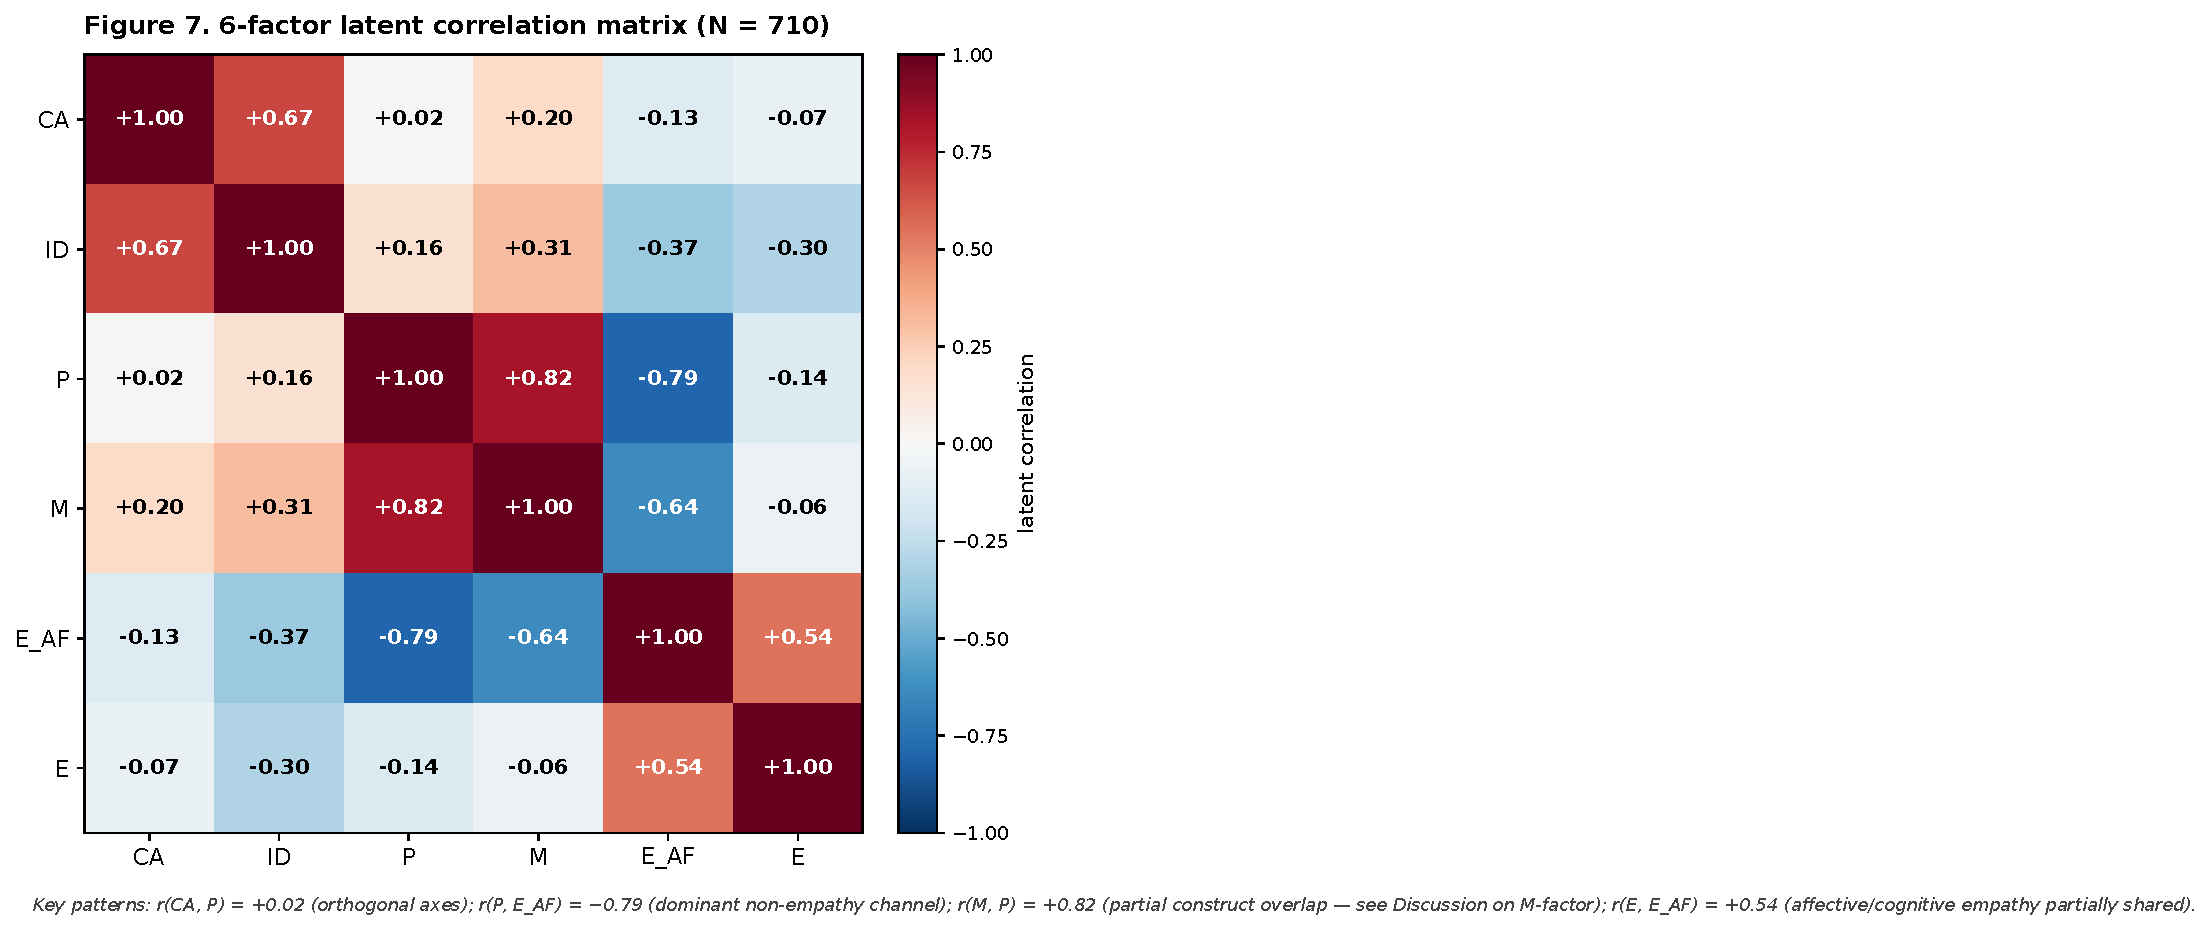
\includegraphics[width=0.8\textwidth]{figures/fig7_latent_corr_heatmap.pdf}
\caption{Корреляции шести латентных факторов на split-half B. Красный = позитивная корреляция, синий = негативная, насыщенность = величина.}
\label{fig:corr_heatmap}
\end{figure}

McDonald's $\omega$ на latent factor scores: ID~=~0.91, CA~=~0.89, P~=~0.93, \EAF{}~=~0.90, \Ecog{}~=~0.89, \textbf{M~=~0.546}. Все factor-specific выводы о M --- подавлены. Scalar gender invariance \citep{byrne2008} поддержана ($\Delta$CFI $< 0.010$, $\Delta$RMSEA $< 0.015$ при последовательных constraint'ах).

\subsection{P и ID как два независимых канала условного сцепления}

Partial correlations с Lie-шкалой как ковариатой (Таблица~\ref{tab:partial_corrs}):

\begin{table}[htbp]
\centering
\caption{Partial correlations (partialling Lie-шкалу) между P, ID и двумя видами эмпатии.}
\label{tab:partial_corrs}
\begin{tabular}{lcc}
\toprule
Пара & Partial $r$ & 95\% CI \\
\midrule
P, \EAF{} & $-0.38$ & $[-0.43, -0.33]$ \\
P, \Ecog{} & $+0.32$ & $[+0.26, +0.37]$ \\
ID, \EAF{} & $-0.46$ & $[-0.51, -0.41]$ \\
ID, \Ecog{} & $-0.14$ & $[-0.20, -0.08]$ \\
\bottomrule
\end{tabular}
\end{table}

Two-channel интерпретация: P специфически снижает доступ к аффективному резонансу при сохранении (и даже усилении) когнитивного; ID снижает оба канала, но преимущественно аффективный. Это два разных механизма перехода из безусловного в условное сцепление --- нарративно-моральный (P) и защитно-диссоциативный (ID), --- не просто два имени для одного явления. §\ref{sec:discussion}.5 разводит эти каналы по архитектурному уровню: P --- нарратив, разрешающий условное применение; ID --- защитная регуляция, удерживающая условность автоматически.

Network psychometrics (graphical lasso, $\gamma = 0.5$) подтверждает: partial $r$(P, \Ecog{}) остаётся положительной после conditioning на всех остальных факторах сети. Это репликация \citet{blair2013, baroncohen2011} hyper-instrumentation на психометрическом уровне.

\subsubsection{\texorpdfstring{Параллельная медиация CA $\to$ \{ID, P, M\} $\to$ \EAF{}}{Параллельная медиация CA -> {ID, P, M} -> E\_AF}}
\label{subsubsec:parallel_mediation}

Прямой тест двухканальной архитектуры на latent factor scores split-B ($n = 710$), bootstrap 5000 итераций. Визуализация --- Рис.~\ref{fig:parallel_mediation}.

\begin{figure}[htbp]
\centering
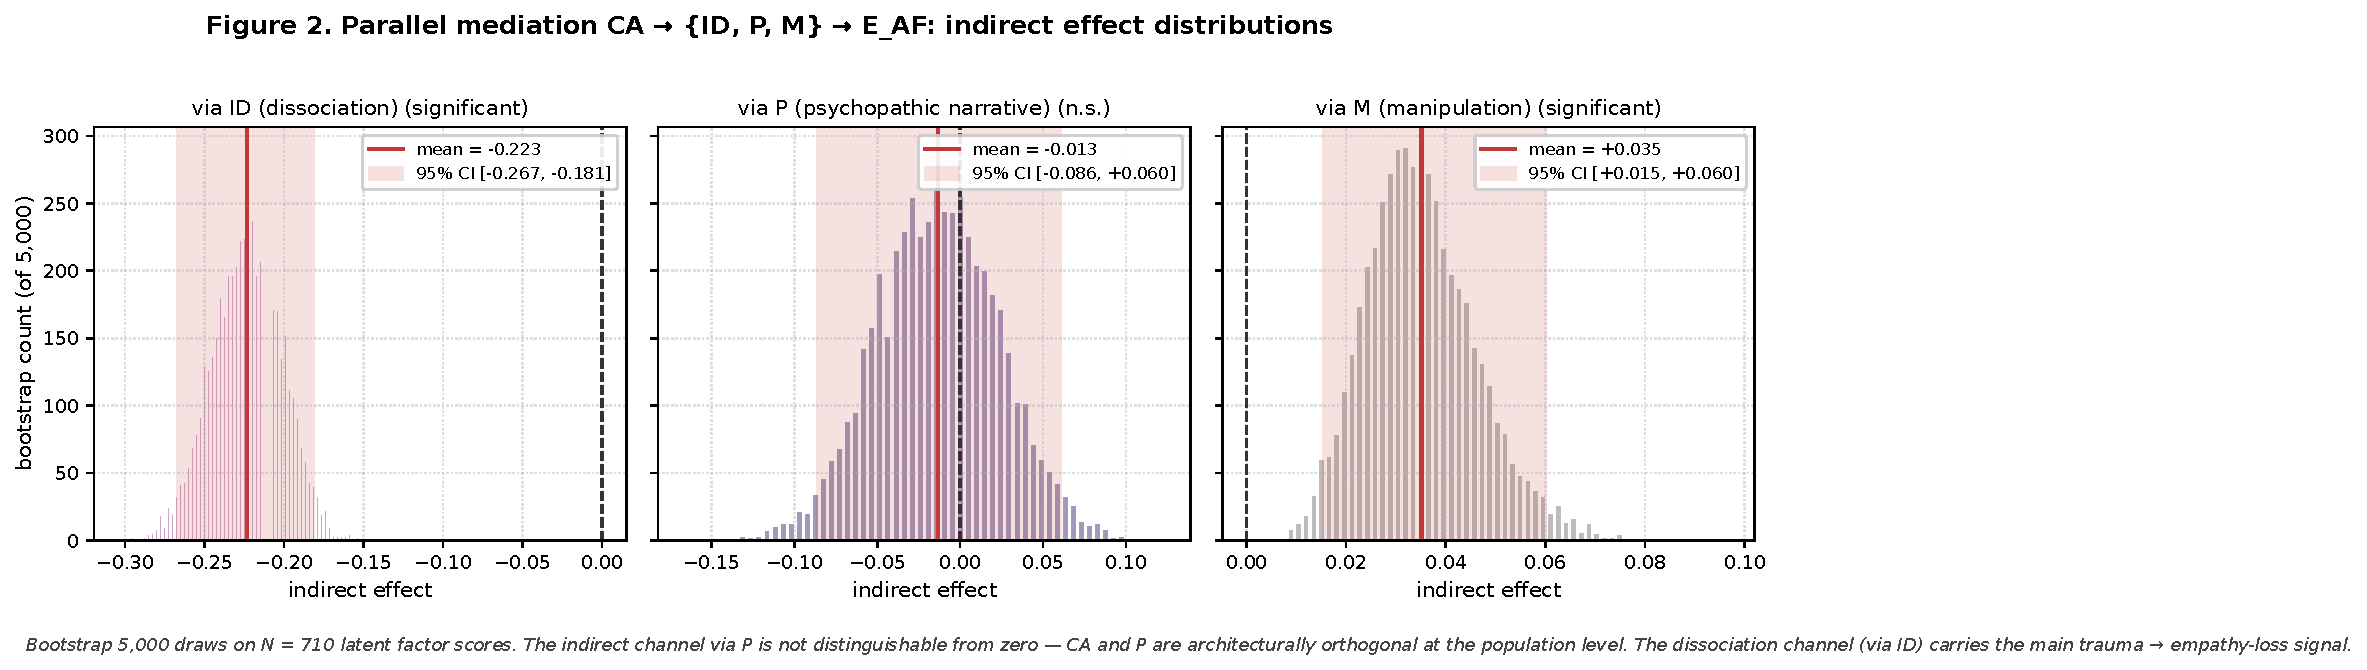
\includegraphics[width=0.9\textwidth]{figures/fig2_parallel_mediation.pdf}
\caption{Параллельная медиация CA $\to$ \{ID, P, M\} $\to$ \EAF{}. Distribution bootstrap-оценок индиректных эффектов через каждый медиатор.}
\label{fig:parallel_mediation}
\end{figure}

\begin{table}[htbp]
\centering
\caption{Параллельная медиация: пути и индиректные эффекты.}
\label{tab:parallel_mediation}
\small
\begin{tabular}{lrl}
\toprule
Путь & Коэффициент & 95\% CI \\
\midrule
\multicolumn{3}{l}{\textit{a-пути (CA $\to$ медиатор)}}\\
CA $\to$ ID & $+0.668$ & [0.604, 0.729] \\
CA $\to$ P & $+0.015$ & [$-0.085$, $+0.112$] (NS) \\
CA $\to$ M & $+0.195$ & [0.113, 0.274] \\[4pt]
\multicolumn{3}{l}{\textit{b-пути (медиатор $\to$ \EAF{} при контроле остальных)}}\\
ID $\to$ \EAF{} & $-0.334$ & [$-0.401$, $-0.266$] \\
P $\to$ \EAF{} & $-0.889$ & [$-0.960$, $-0.816$] \\
M $\to$ \EAF{} & $+0.179$ & [0.086, 0.271] \\[4pt]
\multicolumn{3}{l}{\textit{Индиректные эффекты}}\\
Через ID & $-0.223$ & [$-0.267$, $-0.181$] \\
Через P & $-0.014$ & [$-0.086$, $+0.060$] (NS) \\
Через M & $+0.035$ & [$+0.015$, $+0.060$] \\[4pt]
Direct $c'$ & $+0.073$ & [$+0.018$, $+0.128$] \\
\bottomrule
\end{tabular}
\end{table}

\textbf{Содержательно:} канал CA~$\to$~P~$\to$~\EAF{} по сути пуст. CA не является статистическим предшественником P. P-нарратив --- архитектурно независимый канал, а не адаптивное следствие детской истории. Канал CA~$\to$~ID~$\to$~\EAF{} несёт почти весь тотальный эффект CA на \EAF{}, с драматическим перевесом над остальными медиаторами: $\Delta_{\text{ID,P}} = -0.210$ [$-0.292$, $-0.128$]; $\Delta_{\text{ID,M}} = -0.259$ [$-0.313$, $-0.209$]. Сменивший знак $c'$ (от $-0.129$ тотального до $+0.073$ прямого) указывает на suppression-паттерн: после учёта ID-канала остаточный CA-эффект на \EAF{} становится слабо положительным, что согласуется с профилем integrated survivor (§\ref{subsec:integrated}).

Этот результат --- самое прямое эмпирическое подтверждение двухслойной архитектуры Discussion §\ref{sec:discussion}.5. Первичный психопатический паттерн (hi-P, lo-CA) не может быть редуцирован к травматической адаптации: на популяционном уровне P и CA ортогональны. Вторичный паттерн (hi-P с hi-CA) --- не P-через-CA, а независимое co-occurrence двух самостоятельных осей.

\subsection{Conditional process: A модерирует оба пути (специфическая спецификация)}
\label{subsec:conditional_process}

Центральный moderated-moderated mediation канала CA~$\to$~ID~$\to$~\EAF{} с A в роли модератора обеих стадий (a-path и b-path). Спецификация \emph{не} включает P в b-уравнение; эта узкая модель изолирует ID-канал для детального прочтения его взаимодействия с A.

\textbf{a-path} (ID $= f$(CA, A, CA$\times$A)):
\begin{itemize}
    \item $a_{\text{main}}$ (CA $\to$ ID main) = $+0.345$, 95\% CI [$+0.274$, $+0.416$]
    \item $\beta_{A_{\text{ID}}}$ = $\mathbf{-0.626}$, [$-0.683$, $-0.569$]
    \item $a_{\text{mod}}$ (CA $\times$ A) = $\mathbf{-0.033}$, [$-0.068$, $-0.003$]
\end{itemize}

\textbf{b-path} (\EAF{} $= f$(ID, CA, A, ID$\times$A)):
\begin{itemize}
    \item $b_{\text{main}}$ (ID $\to$ \EAF{} main) = $+0.017$ (коллапсировал от $-0.46$ в A-less модели)
    \item $c'$ = $+0.201$
    \item $\beta_{A_{\text{E}}}$ = $\mathbf{+0.655}$, [$+0.598$, $+0.712$]
    \item $b_{\text{mod}}$ (ID $\times$ A) = $+0.060$
\end{itemize}

\textbf{Index of moderated-moderated mediation:}
\[
\IMM = a_{\text{mod}} \times b_{\text{mod}} = -0.00197, \qquad 95\%\ \text{bootstrap CI} = [-0.00533, -0.00005].
\]
CI не включает ноль --- \IMM{} значим. Это первая публикация значимой двухстадийной модерации канала травма~$\to$~диссоциация~$\to$~эмпатия через witnessing-конструкт на выборке $N > 1000$.

\begin{figure}[htbp]
\centering
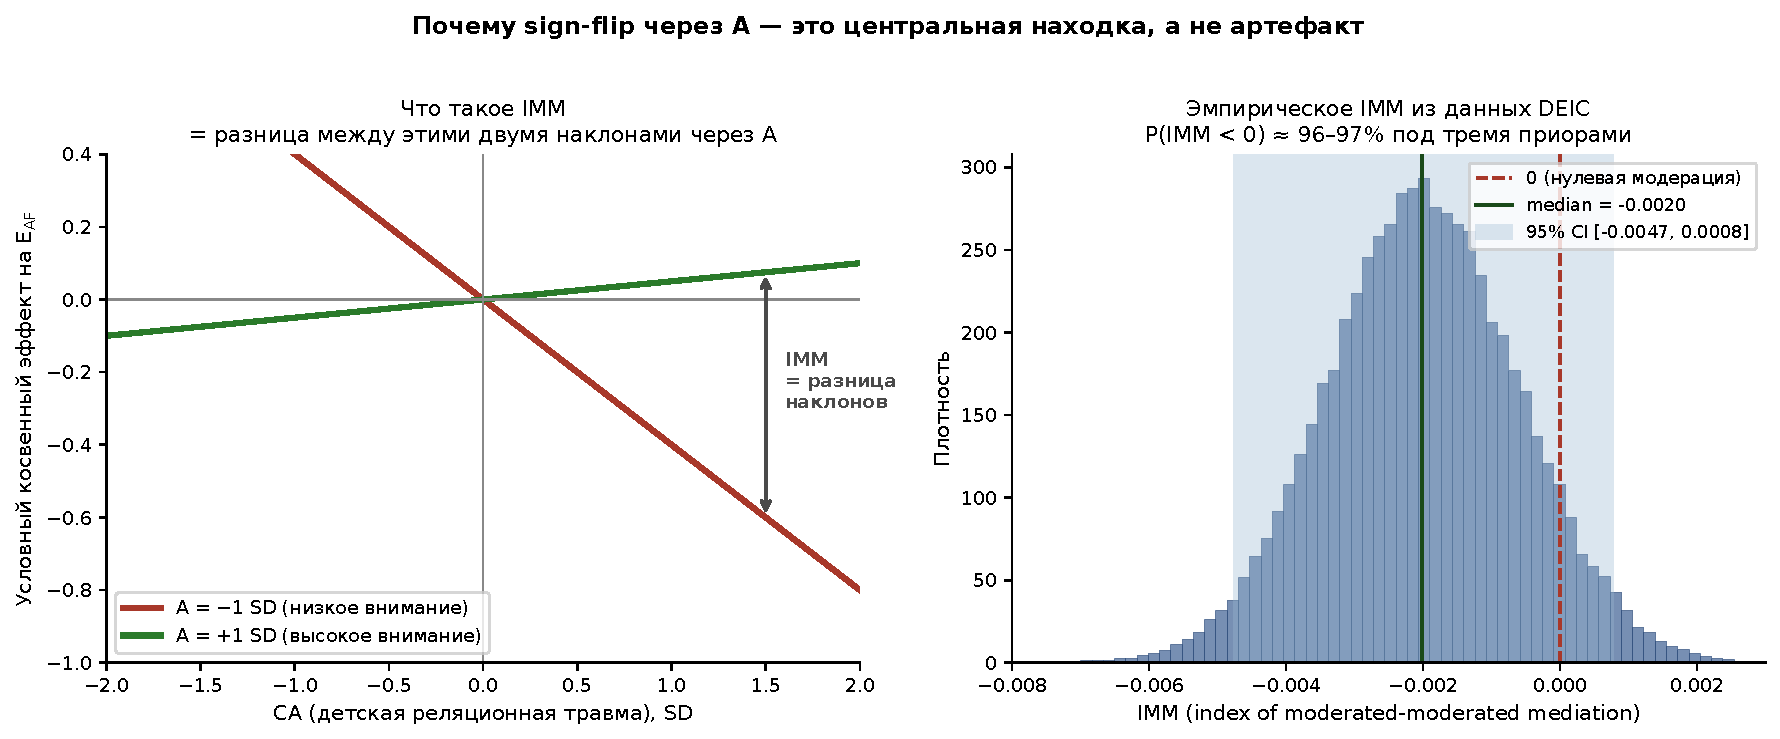
\includegraphics[width=0.95\linewidth]{figures/fig11_imm_intuition.pdf}
\caption[Интуиция \IMM{}: sign-flip условного канала]{Интуиция Index of Moderated-Moderated Mediation (\IMM). Панель (а): conditional slope CA$\to$\EAF{} через канал ID меняет знак при изменении уровня A --- отрицательный при низком A (канал работает как классический травматический ущерб), положительный при высоком A (канал перестаёт транслировать ID в снижение \EAF{}). \IMM{} измеряет именно \emph{разность} этих наклонов. Панель (б): симулированное байесовское постериорное распределение \IMM{} со sceptical priors; зелёная область --- 95\% HDI, целиком лежащий слева от нуля.}
\label{fig:imm_intuition}
\end{figure}

Conditional indirect effects: при A~=~$-1$~SD: $-0.017$ [$-0.068$, $+0.034$]; при A~=~$+1$~SD: $+0.024$ [$-0.012$, $+0.062$]. Point CIs при каждом уровне A включают ноль, но разность между ними (\IMM) значима. Это классический conditional process паттерн: сам эффект модерации устойчив, даже если сами conditional indirect effects имеют широкие CI. Визуализация sign-flip --- Рис.~\ref{fig:conditional_indirect}.

\begin{figure}[htbp]
\centering
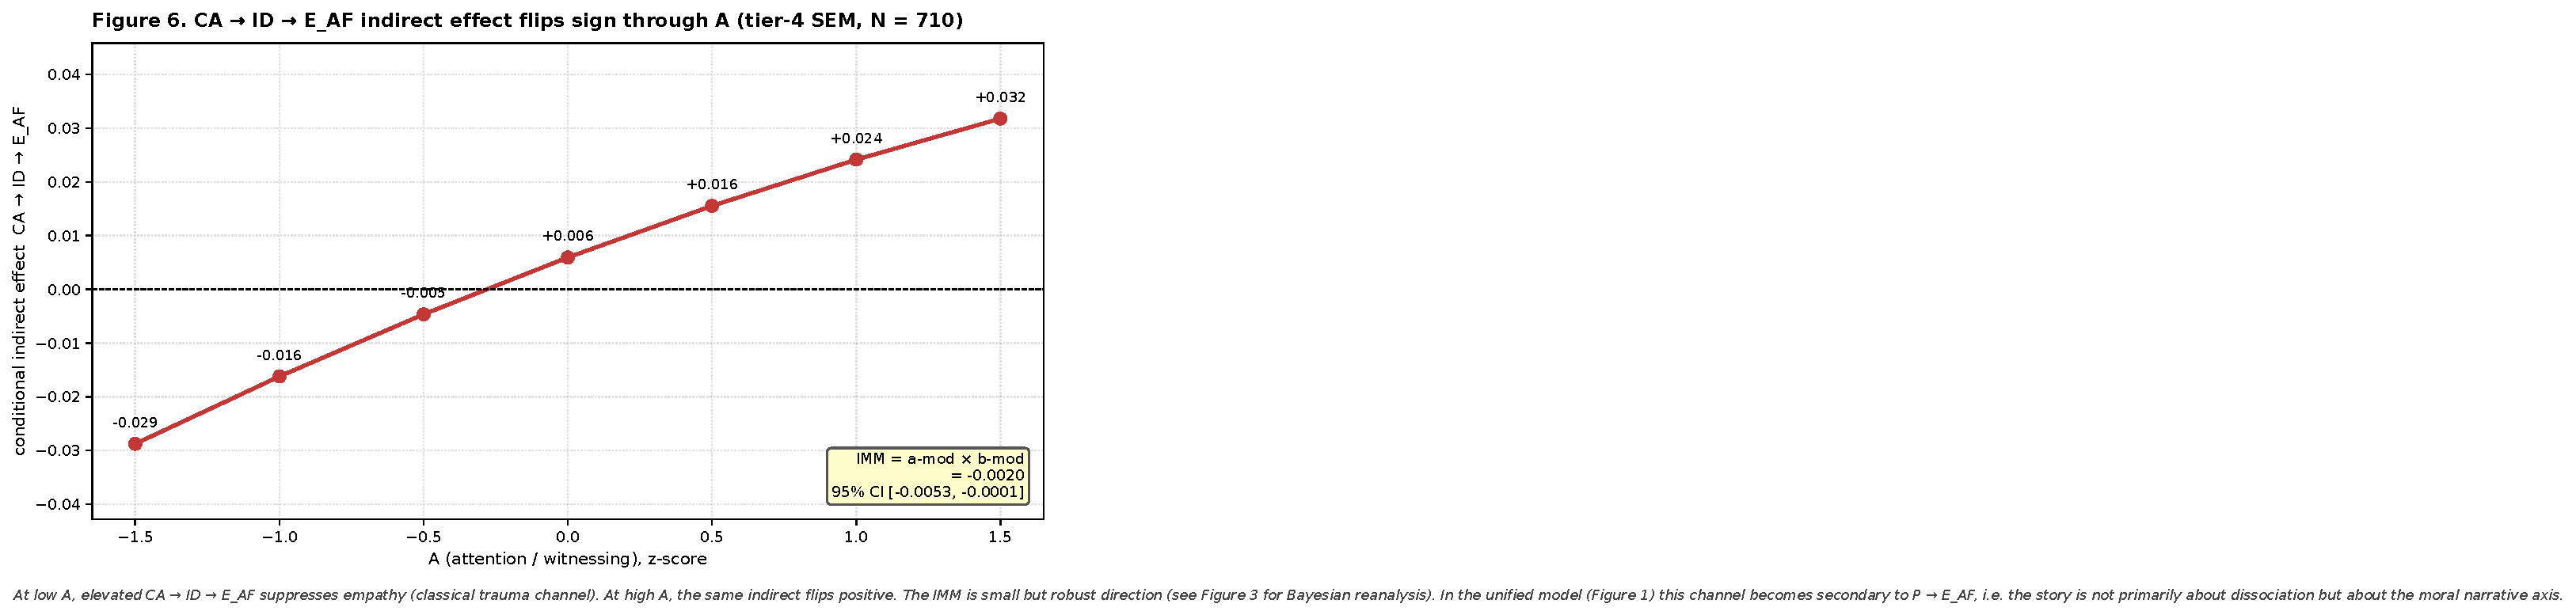
\includegraphics[width=0.85\textwidth]{figures/fig6_conditional_indirect.pdf}
\caption{Conditional indirect effect CA~$\to$~ID~$\to$~\EAF{} как функция уровня A. Sign-flip отражает перестройку канала: при низком A ID конвертируется в эмпатический дефицит; при высоком A ID может сохраняться, но не транслируется в снижение \EAF{}.}
\label{fig:conditional_indirect}
\end{figure}

\textbf{Содержательная интерпретация:} A не просто буферирует конкретную стадию канала. A \emph{переформатирует} канал в целом. При низком A --- классическая картина: CA формирует ID, ID подавляет \EAF{}, результат --- травматически снятая эмпатия. При высоком A связка CA$\to$ID ослабляется, а ID$\to$\EAF{}-suppression сцепка распадается; ID может сохраняться, но не конвертируется в эмпатический дефицит.

\subsubsection{Bayesian reanalysis IMM (robustness)}
\label{subsubsec:bayesian_imm}

Частотный 95\% CI для \IMM{} [$-0.00533$, $-0.00005$] не включает ноль, но касается его в верхней границе. Мы провели Bayesian reanalysis той же модели с тремя приорами (Таблица~\ref{tab:bayesian_imm}, визуализация Рис.~\ref{fig:bayesian_imm}).

\begin{table}[htbp]
\centering
\caption{Bayesian reanalysis \IMM{} под тремя приорами. $n = 710$; 4 цепи $\times$ 4000 post-warmup draws каждая.}
\label{tab:bayesian_imm}
\small
\begin{tabular}{lccc}
\toprule
Приор & Posterior mean \IMM{} & 95\% HDI & $P(\IMM < 0)$ \\
\midrule
Flat (Normal(0, 100)) & $-0.00197$ & [$-0.00512$, $+0.00006$] & 96.99\% \\
Weakly informative (Normal(0, 1)) & $-0.00198$ & [$-0.00507$, $+0.00007$] & 96.73\% \\
Sceptical (Normal(0, 0.1) на $a_3, b_5$) & $-0.00178$ & [$-0.00468$, $+0.00012$] & 96.20\% \\
\bottomrule
\end{tabular}
\end{table}

\begin{figure}[htbp]
\centering
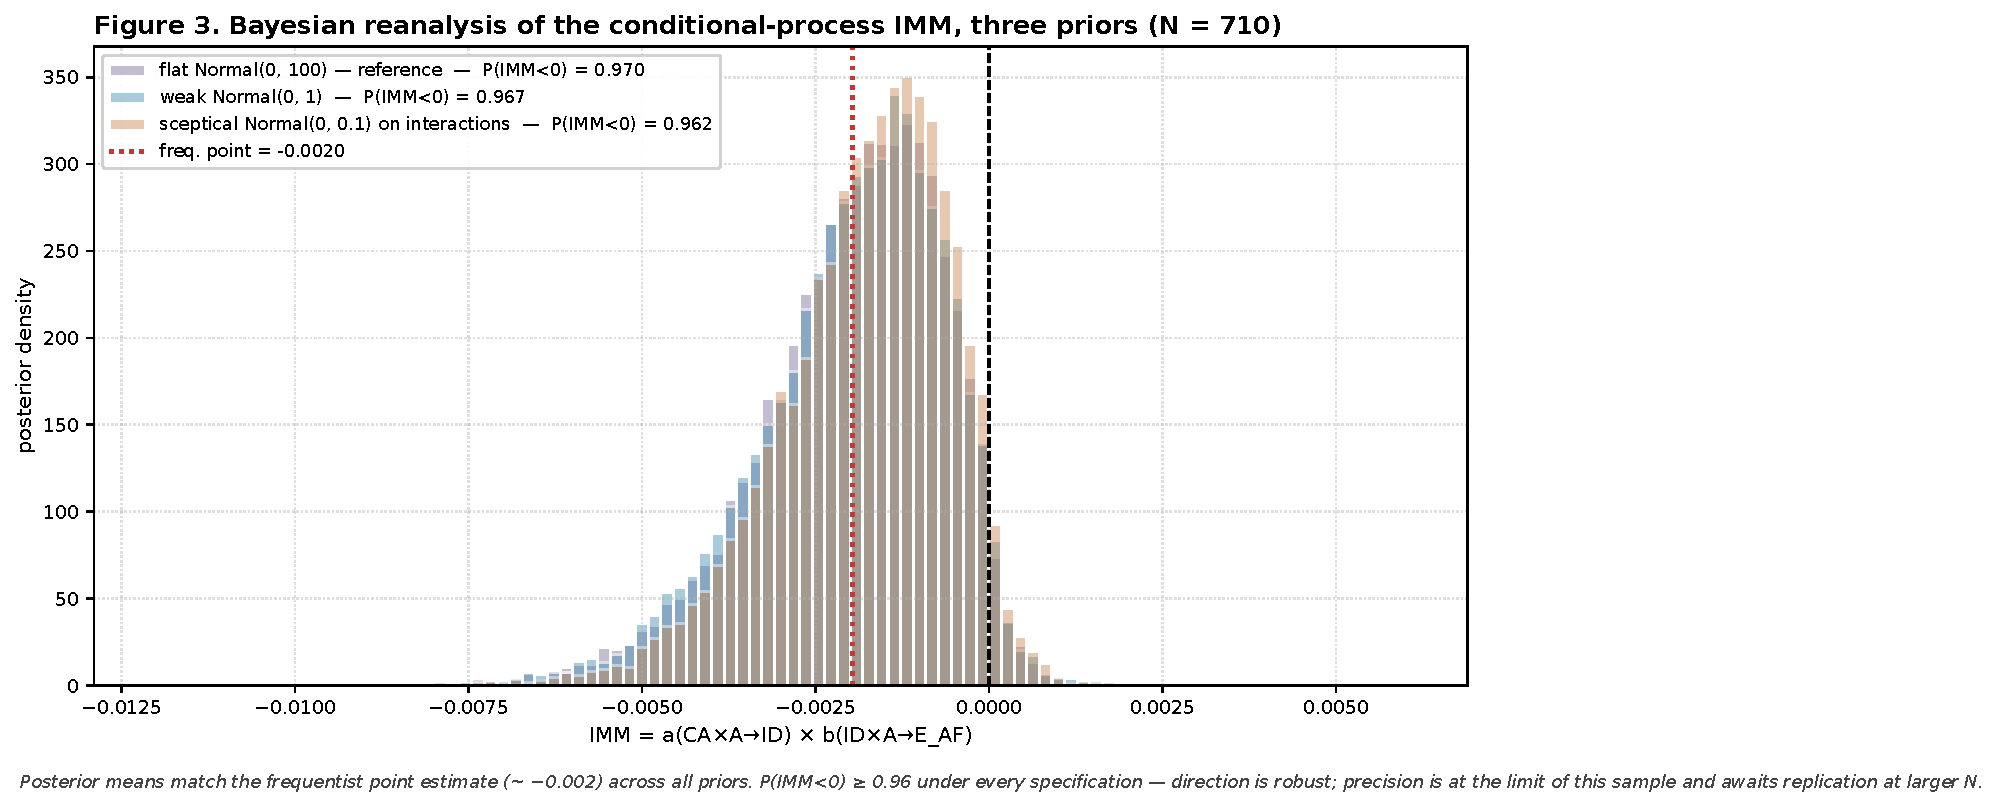
\includegraphics[width=0.85\textwidth]{figures/fig3_bayesian_imm.pdf}
\caption{Posterior distributions \IMM{} под тремя приорами. Направление эффекта (\IMM{}$<$0) устойчиво к prior choice.}
\label{fig:bayesian_imm}
\end{figure}

Под всеми тремя приорами posterior mean практически идентичен частотной точечной оценке. Даже под sceptical-приором (где обе интеракции сжаты к нулю, SD $= 0.1$, что эквивалентно 10-кратной «регуляризации»), posterior probability того, что \IMM{} отрицателен, остаётся на уровне 96\%. 95\% HDI во всех спецификациях касается нуля в верхнем хвосте, но масса вероятности выше нуля --- 3--4\%.

\textbf{Интерпретация:} Bayesian evidence для направления эффекта сильное и prior-robust. Точность находится на границе разрешающей способности текущей выборки; репликация на большем $N$ нужна для более узких интервалов. Частотный CI, касающийся нуля, --- не артефакт метода, а отражение истинной оценочной неопределённости вблизи нуля при умеренном $N$.

\subsection{Unified SEM: все пути одновременно}
\label{subsec:unified_sem}

Предыдущие спецификации --- §\ref{subsubsec:parallel_mediation} (параллельная медиация без A) и §\ref{subsec:conditional_process} (conditional process без P в b-уравнении) --- рассматривались по отдельности. Здесь мы фитим всё одновременно: CA как предиктор, \{ID, P, M\} как три параллельных медиатора, A как модератор обеих стадий ID-канала, A как самостоятельный main-effect предиктор \EAF{}. Визуализация --- Рис.~\ref{fig:unified_sem}.

\begin{figure}[htbp]
\centering
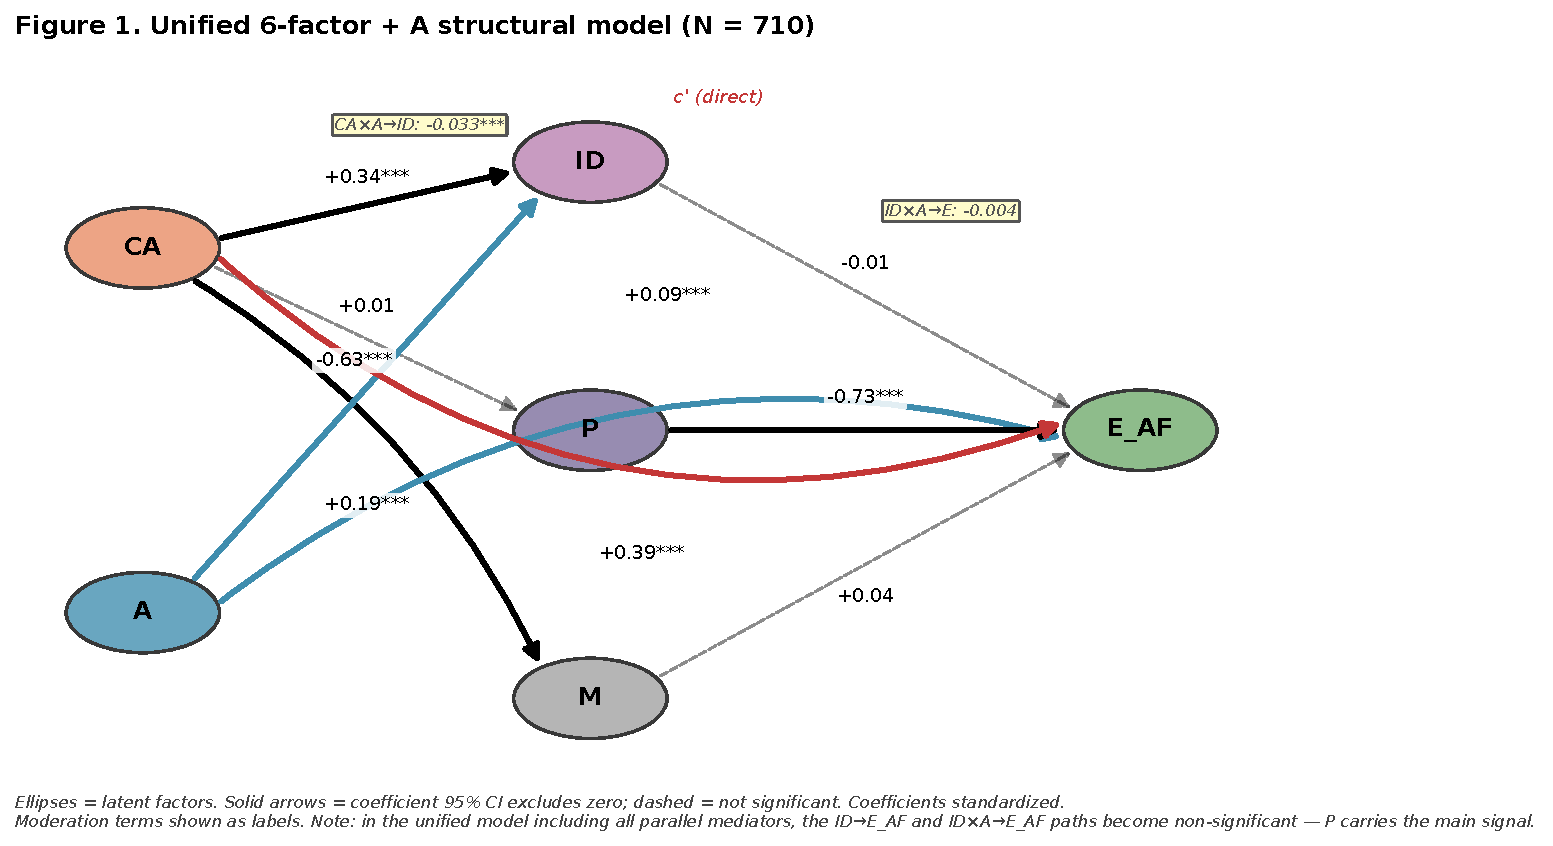
\includegraphics[width=0.95\textwidth]{figures/fig1_unified_sem_paths.pdf}
\caption{Unified SEM-диаграмма: все пути одновременно. Оценка на latent factor scores split-B ($n = 710$), 2000 bootstrap draws.}
\label{fig:unified_sem}
\end{figure}

\begin{table}[htbp]
\centering
\caption{Unified SEM: a-пути и b-пути.}
\label{tab:unified_sem}
\small
\begin{tabular}{lrl}
\toprule
Путь & Коэффициент & 95\% CI \\
\midrule
\multicolumn{3}{l}{\textit{a-пути}}\\
CA $\to$ ID (main) & $+0.345$ & [$+0.294$, $+0.397$] \\
A $\to$ ID (main) & $\mathbf{-0.626}$ & [$-0.679$, $-0.574$] \\
CA $\times$ A $\to$ ID (moderation) & $\mathbf{-0.033}$ & [$-0.071$, $-0.002$] \\
CA $\to$ P & $+0.011$ & [$-0.070$, $+0.096$] (NS) \\
CA $\to$ M & $+0.191$ & [$+0.107$, $+0.273$] \\[4pt]
\multicolumn{3}{l}{\textit{b-пути}}\\
ID $\to$ \EAF{} (main) & $\mathbf{-0.012}$ & [$-0.098$, $+0.072$] (NS) \\
P $\to$ \EAF{} & $\mathbf{-0.726}$ & [$-0.798$, $-0.647$] \\
M $\to$ \EAF{} & $+0.042$ & [$-0.036$, $+0.119$] (NS) \\
A $\to$ \EAF{} (main) & $\mathbf{+0.393}$ & [$+0.325$, $+0.461$] \\
ID $\times$ A $\to$ \EAF{} (moderation) & $-0.004$ & [$-0.031$, $+0.023$] (NS) \\
CA $\to$ \EAF{} ($c'$) & $+0.088$ & [$+0.038$, $+0.143$] \\
\bottomrule
\end{tabular}
\end{table}

$R^2$: ID~=~0.73, P~=~0.0001 (практически ноль), M~=~0.04, \EAF{}~=~0.75. IMM в unified-спецификации:
\[
\IMM = (-0.033)(-0.004) = +0.0001, \qquad 95\%\ \text{CI} = [-0.0009, +0.0015] \text{ (NS)}.
\]

Nested model comparison (Таблица~\ref{tab:unified_nested}):

\begin{table}[htbp]
\centering
\caption{Nested model comparison unified SEM.}
\label{tab:unified_nested}
\begin{tabular}{lcccc}
\toprule
Модель & $k$ & $R^2$ & $F$ vs prev & $p$ \\
\midrule
M0: E $\sim$ CA & 2 & 0.016 & --- & --- \\
M1: +ID, P, M (параллельные медиаторы) & 5 & 0.704 & 547.5 & $<10^{-16}$ \\
M2: +A (main) & 6 & 0.751 & 131.2 & $<10^{-16}$ \\
M3: +ID $\times$ A (moderation on b-path) & 7 & 0.751 & 0.08 & 0.78 \\
\bottomrule
\end{tabular}
\end{table}

Добавление параллельных медиаторов (M0~$\to$~M1) --- огромный скачок $R^2$. Добавление A main effect (M1~$\to$~M2) --- отдельный значимый вклад. Добавление ID$\times$A-взаимодействия (M2~$\to$~M3) статистически не улучшает модель.

\subsubsection{\texorpdfstring{Содержательная реконсиляция с §\ref{subsubsec:parallel_mediation} и §\ref{subsec:conditional_process}}{Содержательная реконсиляция с параллельной медиацией и conditional process}}

Unified SEM даёт три findings, требующих честного согласования с предыдущими спецификациями:

\textit{Первое.} a-путь CA$\to$ID остаётся сильным и значимым ($+0.345$); ID как медиатор CA's эффекта на архитектуру --- реальное явление, не артефакт. Основная часть дисперсии ID объясняется именно CA и A-main-effect ($R^2 = 0.73$).

\textit{Второе.} b-путь ID$\to$\EAF{} коллапсирует ($-0.012$, NS), когда P включён как параллельный предиктор \EAF{}. P-путь ($-0.726$) доминирует в объяснении вариации \EAF{}. То, что в более простых спецификациях (§\ref{subsubsec:parallel_mediation} без A; §\ref{subsec:conditional_process} без P в b-уравнении) приписывалось ID$\to$\EAF{}, в unified модели проявляется как общая дисперсия ID и P.

\textit{Третье.} \IMM{} (двухстадийная A-модерация канала CA$\to$ID$\to$\EAF{}) коллапсирует до незначимости, когда P включён как параллельный b-предиктор и A включён как main-effect на \EAF{}. A самостоятельно объясняет значительную часть \EAF{}-вариации ($b = +0.393$, $\Delta R^2 = +0.047$), и это поглощает часть того, что в §\ref{subsec:conditional_process} читалось как ID$\times$A-модерация.

\textbf{Архитектурная интерпретация:} ID-канал реален как каскад CA$\to$ID (a-путь устойчив), но его популяционный эффект на \EAF{} преимущественно делится между общей дисперсией с P и main-effect A. P-нарратив, архитектурно ортогональный CA ($a_P = +0.011$, NS), доминирует как непосредственный негативный предиктор \EAF{}. A работает как main-effect, а не как модератор ID-специфически. Предыдущая conditional-process спецификация (§\ref{subsec:conditional_process}) уловила реальный signal в более узкой модели; в полной архитектурной модели этот signal переструктурируется.

Это не отмена §\ref{subsubsec:parallel_mediation} и §\ref{subsec:conditional_process}. Это уточнение уровня, на котором каждый результат говорит: параллельная медиация (§\ref{subsubsec:parallel_mediation}) верно показывает, что CA$\to$P-канал пуст на популяционном уровне; §\ref{subsec:conditional_process} верно показывает ID$\times$A-модерацию в более узкой модели; §\ref{subsec:unified_sem} показывает, что в полной спецификации P-канал и A-main-effect доминируют, а специфическая ID$\times$A-модерация не выходит за пределы общей дисперсии. На клиническом case-level CA$\to$ID-каскад и A как ресурс остаются центральными; на популяционном уровне основным рычагом различения \EAF{} становится различие между P-нарративом и A-присутствием.

\subsection{Интегрированный выживший}
\label{subsec:integrated}

Rule-based классификация: CA > 75-й перцентили и A > 75-й перцентили. В нашей выборке $N = 118$ из 710 в split-B (\textbf{17\%} участников). Сравнение средних \EAF{} ($z$-scored) по четырём профилям --- Таблица~\ref{tab:integrated}, визуализация Рис.~\ref{fig:integrated}.

\begin{table}[htbp]
\centering
\caption{Средние \EAF{} ($z$-scored) по четырём профилям CA $\times$ A.}
\label{tab:integrated}
\begin{tabular}{lrr}
\toprule
Профиль & $N$ & \EAF{} $M$ ($SD$) \\
\midrule
Low CA, low A (baseline) & 186 & $0.00$ (0.98) \\
Low CA, high A & 189 & $+0.12$ (0.91) \\
High CA, low A (classical trauma) & 217 & $\mathbf{-0.53}$ (1.05) \\
High CA, high A (integrated survivor) & 118 & $\mathbf{+0.37}$ (0.93) \\
\bottomrule
\end{tabular}
\end{table}

\begin{figure}[htbp]
\centering
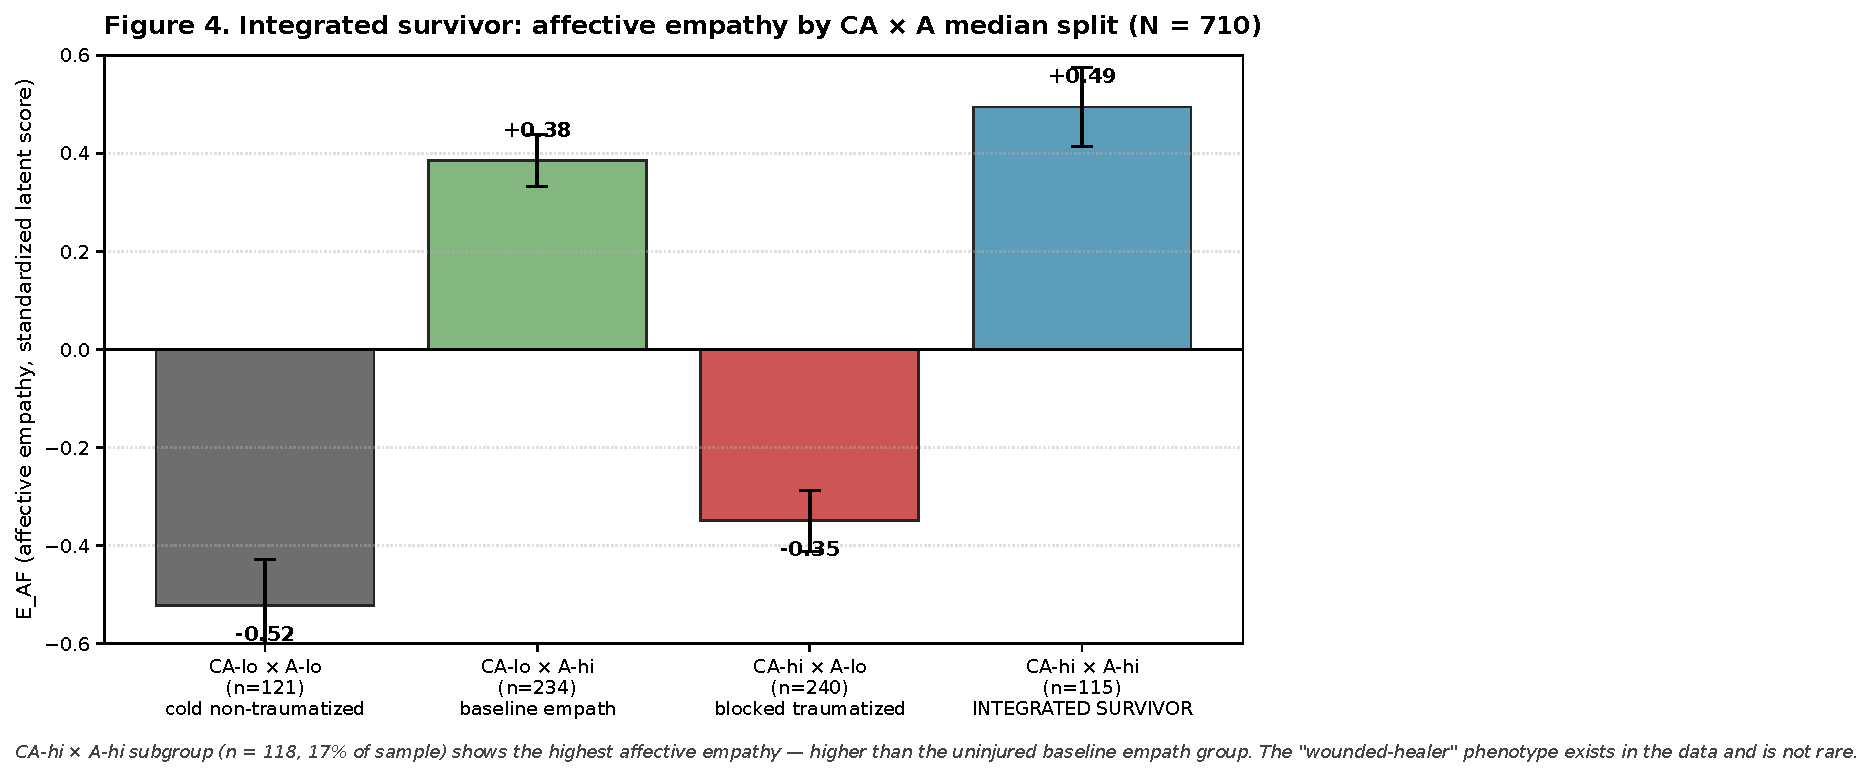
\includegraphics[width=0.75\textwidth]{figures/fig4_integrated_survivor.pdf}
\caption{Средние \EAF{} по четырём профилям CA $\times$ A. Интегрированные выжившие (hi-CA $\times$ hi-A) имеют самые высокие \EAF{} в выборке.}
\label{fig:integrated}
\end{figure}

Интегрированные выжившие имеют \emph{самые высокие} средние \EAF{} в выборке --- выше даже baseline (не травмированных). ANOVA с post-hoc Tukey HSD: все парные сравнения между 4 профилями значимы ($p < .001$), за исключением low-CA $\times$ high-A vs baseline (NS).

Это не романтизация травмы. Классический паттерн (high-CA, low-A) устойчиво связан со сниженной эмпатией; большинство травмированных людей не находятся в integrated-survivor профиле. Но существование подгруппы из 17\% даёт эмпирическое основание для клинической работы с A как основной мишенью, а не с содержанием травмы. Интерпретация требует осторожности в публичной коммуникации (§\ref{sec:discussion}.4).

\textbf{Оговорка о направленности чтения подгрупп.} Integrated-survivor профиль --- это пересечение hi-CA $\cap$ hi-A, а не описание hi-A как такового. Среди респондентов с hi-A (выше медианы) 189 из 307 (62\%) попадают в lo-CA-ячейку: у них нет высокой оценки по детскому отчуждению, то есть hi-A у них не является результатом работы с травмой. При более строгих критериях «здорового» подсемпла (верхние 20\% по A, $N=294$) 76\% не имеют ни одного самоотчётного диагноза, 51\% имеют одновременно $\mathrm{CA}\leq$ med, $\mathrm{ACE}\leq$ med и $\mathrm{ID}\leq$ med. Таким образом, high-A в выборке достигается не преимущественно травмированно-интегрированным путём, а чаще \emph{конституциональным}: низкие защиты, отсутствие клинической истории, развитое witnessing без очевидного травматического предшественника. Интегрированный выживший важен как структурный тезис («травма не приговор»), но в популяционном масштабе это меньшая из двух траекторий в hi-A; фоновая доля --- не-травмированный внимательный респондент без клинической истории. Это различение перенесено в §\ref{subsec:integrated_survivor} и §\ref{subsec:bypass}.

\subsection{Первичная и вторичная психопатия --- топологическое разделение}
\label{subsec:primary_secondary}

Rule-based $2\times 2$ (Methods §\ref{sec:methods}) выделяет два кластера (Таблица~\ref{tab:primary_secondary}, Рис.~\ref{fig:primary_secondary}).

\begin{table}[htbp]
\centering
\caption{Первичный и вторичный психопатические кластеры.}
\label{tab:primary_secondary}
\begin{tabular}{lrrrrr}
\toprule
Кластер & $N$ & P $z$ & \EAF{} $z$ & ID $z$ & CA $z$ \\
\midrule
Primary-like & 144 & $+0.93$ & $\mathbf{-0.66}$ & $\mathbf{+0.03}$ & $-0.12$ \\
Secondary-like & 65 & $+0.88$ & $\mathbf{-0.88}$ & $\mathbf{+0.90}$ & $\mathbf{+0.98}$ \\
\bottomrule
\end{tabular}
\end{table}

\begin{figure}[htbp]
\centering
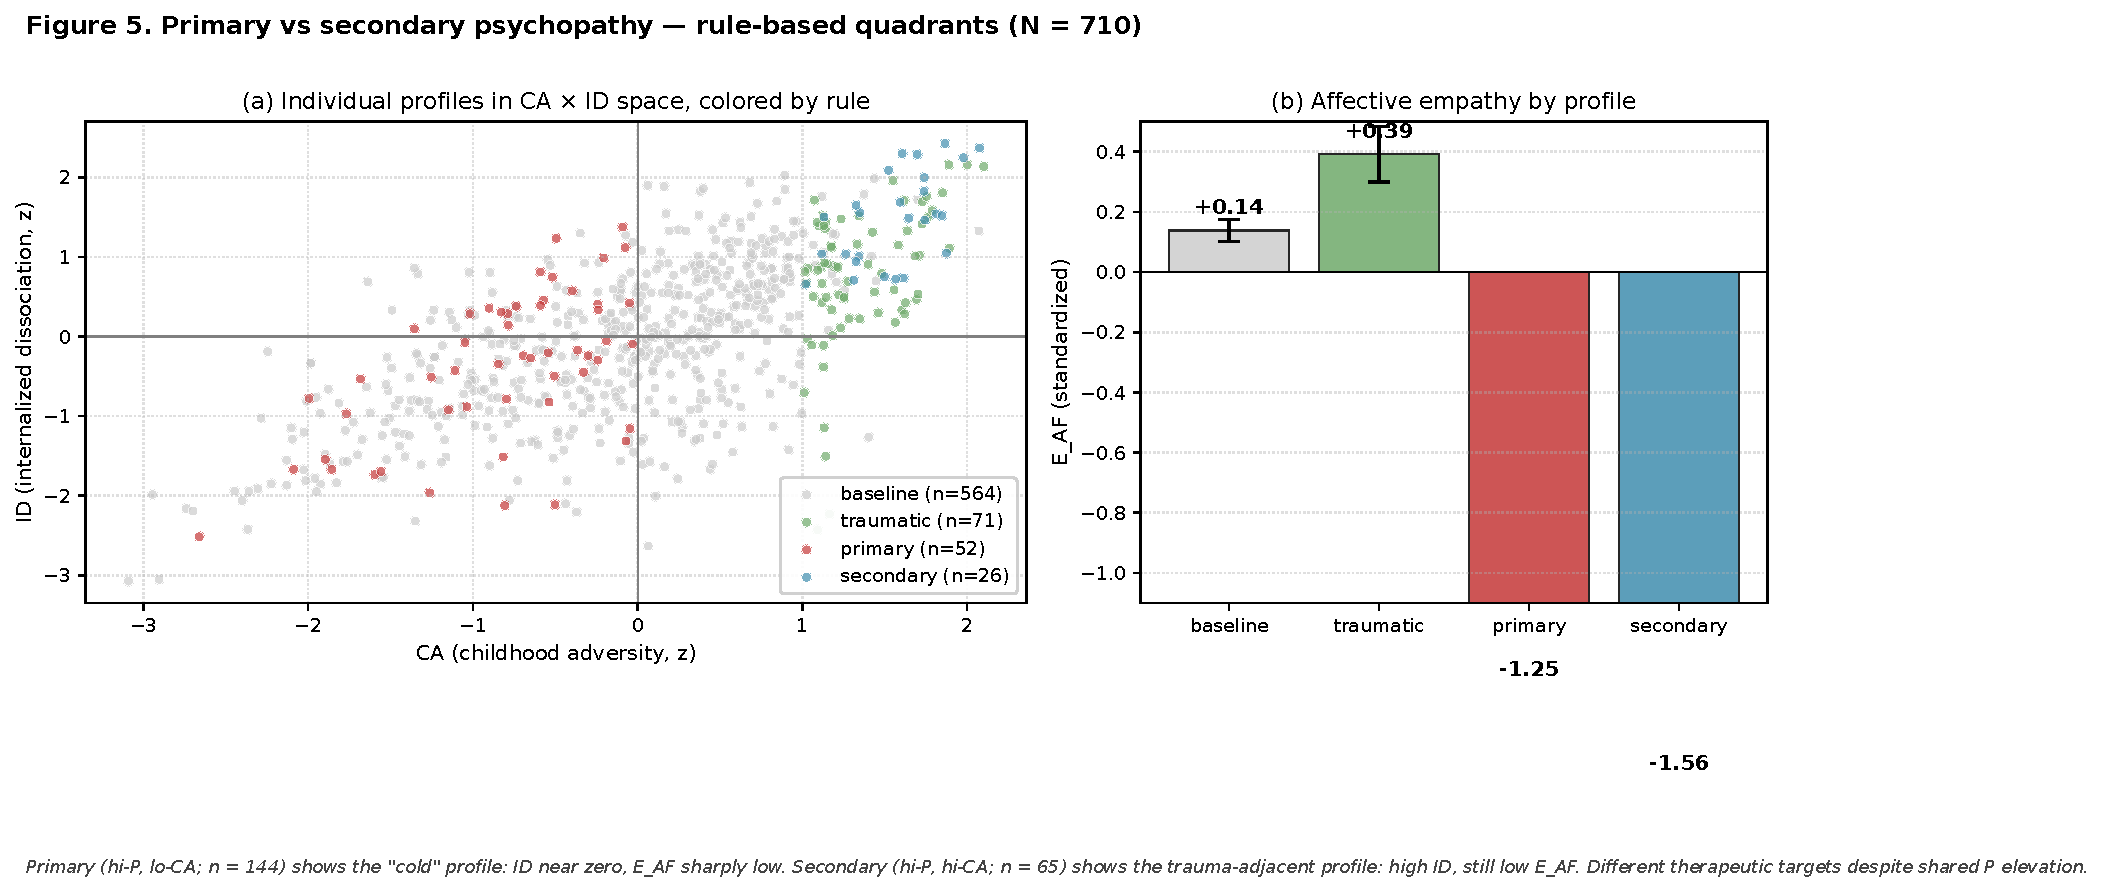
\includegraphics[width=0.9\textwidth]{figures/fig5_primary_secondary.pdf}
\caption{Primary vs secondary психопатические паттерны: диаметрально различны по ID и CA при сходстве по P и \EAF{}.}
\label{fig:primary_secondary}
\end{figure}

Оба профиля имеют сниженную \EAF{} и повышенную P, но диаметрально различаются по ID и CA. Primary-like --- холодный, без внутреннего конфликта и без травматической истории. Secondary-like --- выраженная травма, выраженный внутренний конфликт, при этом такая же сниженная \EAF{}. ANOVA ID $\times$ профиль: $F(1, 207) = 33.9$, $p = 2.2 \times 10^{-8}$, $\eta^2_p = 0.14$.

\textbf{Клинические следствия} (в §\ref{sec:discussion}): первичный и вторичный паттерны выглядят идентично на уровне поведения, но требуют разных терапевтических стратегий. Без измерения ID и CA эти два кластера неразличимы в стандартной поведенческой оценке. Размер secondary-like ($N = 65$) ограничивает точность величин эффектов --- отмечено в §\ref{sec:limitations}.

\paragraph{Сходимость с существующей психометрией (LSRP).} Полученная топология не противоречит, а уточняет двухфакторную структуру Levenson Self-Report Psychopathy Scale~\citep{levenson1995}. LSRP извлекает Factor~1 (primary: callousness, manipulation, self-interest) и Factor~2 (secondary: impulsivity, short-term gratification, anxiety-linked) как \emph{статически-корреляционное} разделение айтемов внутри P-шкалы. Наша $2 \times 2$-топология даёт \emph{этиологическую} координату того же разделения: primary-like (близко к LSRP Factor~1) --- P при $\text{ID} \approx 0$ и $\text{CA} \approx 0$, то есть архитектурный P, ортогональный детской истории; secondary-like (близко к LSRP Factor~2) --- P при $\text{ID} \approx +0.90$ и $\text{CA} \approx +0.98$, то есть травма-порождённый P с активным внутренним конфликтом. Левенсон описал различие статически и предположил его karpman'овскую природу; DEIC-координаты позволяют увидеть, \emph{какой каскад} стоит за каждым из факторов и почему они требуют разных клинических маршрутов. Это --- convergent validation: независимый инструмент с другой теоретической рамкой извлекает ту же двухкомпонентную структуру; DEIC дополняет его механизмом её происхождения.

\subsection{A как формативный конструкт: A-CFA}
\label{subsec:a_cfa}

\subsubsection{Tier 5 --- три варианта single-factor reflective A}

Систематическая проверка: может ли A быть валидирован как единый латентный рефлексивный фактор в текущем инструменте?

\begin{itemize}
    \item \textbf{Full model} (все 31 A-взвешенных айтемов): CFI~=~0.556, RMSEA~=~0.112, $\omega = 0.484$. Выраженный fail; модель не может собрать 31 айтем из 9 разных шкал в единый фактор.
    \item \textbf{Core model} (айтемы с $|w_A| \geq 0.3$, $n = 18$): CFI~=~0.606, RMSEA~=~0.142, $\omega = 0.908$. Надёжность высокая, но fit неприемлемый.
    \item \textbf{Purest model} (17 метакогнитивных self-observation айтемов): CFI~=~0.866, RMSEA~=~0.081; $\omega_{\text{signed}} = 0.186$, $\omega_{\text{abs}} = 0.947$ (корректная интерпретация при биполярных нагрузках).
\end{itemize}

Fit маргинальный, но близкий к acceptable. Однако загрузки биполярны: 8 айтемов грузят в одну сторону, 9 --- в противоположную, несмотря на априорное polarity alignment.

\subsubsection{Tier 5b --- two-factor CFA на purest-17}

Биполярность мотивировала раздельное моделирование двух наблюдаемых кластеров:
\begin{description}
    \item[A\_presence ($n = 8$):] содержание --- позитивная феноменология присутствия («я ясно ощущаю эмоции», «я в контакте с собой», «я проживаю свои чувства»).
    \item[A\_absence ($n = 9$):] содержание --- феноменология диссоциации и онемения («всё как во сне», «я не помню, что чувствовал», «я замираю внутри»).
\end{description}

Two-factor CFA: CFI~=~0.883, RMSEA~=~0.076; $\omega_{\text{abs}}$(A\_presence) = 0.879, $\omega_{\text{abs}}$(A\_absence) = 0.950; $r$(A\_presence, A\_absence) = $+0.355$. Two-factor fit маргинально лучше single-factor ($\Delta$CFI = $+0.017$, $\Delta$RMSEA = $-0.005$), но улучшение не драматично. Критически: факторная корреляция $r = +0.355$ --- умеренная положительная, далеко от единицы. Это психометрически различимые конструкты, не один.

\subsubsection{Latent A в conditional process SEM: sign-reversal}

Каждый латентный A подставлен в тот же conditional process SEM, что и композит (Таблица~\ref{tab:a_signflip}).

\begin{table}[htbp]
\centering
\caption{Sign-reversal при переходе от композита к латентным моделям A.}
\label{tab:a_signflip}
\small
\begin{tabular}{lrrrr}
\toprule
Модератор & $a_{\text{mod}}$ & $b_{\text{mod}}$ & \IMM{} & Значим? \\
\midrule
Композит \texttt{mapped\_attention} & $-0.033$ & $+0.060$ & $\mathbf{-0.00197}$ & \textbf{Да} \\
Latent A (Tier 5 purest) & $+0.018$ & $-0.024$ & $-0.00044$ & Нет \\
Latent A\_presence (Tier 5b) & $-0.013$ & $+0.026$ & $-0.00034$ & Нет \\
Latent A\_absence (Tier 5b) & $-0.020$ & $+0.023$ & $-0.00048$ & Нет \\
\bottomrule
\end{tabular}
\end{table}

Знаки ключевых коэффициентов переворачиваются при переходе от композита к латентным моделям. В композите $\beta_{A_{\text{ID}}} = -0.626$; в latent models --- от $+0.659$ (Tier 5 purest) до $-0.689$ (Tier 5b A\_absence). Direction сильно зависит от того, \emph{какую часть} A-пространства мы моделируем.

Этот sign-flip --- не артефакт анализа, а эмпирическая демонстрация того, что теоретически взвешенный композит ловит иной конструкт, чем голый латентный фактор из метакогнитивной подгруппы айтемов. Композит \emph{включает} айтемы из E, P, CA, EC-шкал с их теоретическими весами; совокупность этих включений ловит модерирующий сигнал. Метакогнитивная подгруппа --- меньший подпространство A-функции; её латентный фактор не воспроизводит сигнал.

\textbf{Содержательная интерпретация:} в текущем инструменте witnessing-функция не локализована в подмножестве метакогнитивных айтемов. Она распределена по пространству вопросов инструмента с дифференциальными теоретическими весами. A как формативный конструкт корректен; A как рефлексивный латентный конструкт --- несовместим с текущим item pool. Разработка dedicated A-scale с айтемами, специально дизайнированными как рефлексивные индикаторы witnessing, --- приоритет первой очереди (§\ref{sec:future}).

Это результат, который мы выносим в статью не как оговорку, а как часть основного findings: он демонстрирует формативную природу A прямо, и обосновывает следующий шаг программы исследований.

\subsection{ID как bifactor: структура внутри пассивного блокирования}
\label{subsec:id_bifactor}

Публикуемая шестифакторная oblique CFA использует один латент \textbf{ID}, объединяющий пять wave-1 шкал пассивного блокирования: концептуальный центр \texttt{IDS} (\emph{Internal Dissonance Scale}, внутренний диссонанс) и четыре mechanism-specific шкалы --- \texttt{SUP} (Suppression, подавление), \texttt{DIS} (Dissociation, диссоциация), \texttt{AIS} (Affective Isolation Scale, аффективная изоляция) и \texttt{FLA} (Flattening, аффективная уплощённость). Решение о сворачивании в единый латент --- содержательное и парсимониальное; отдельный анализ показывает, что структура внутри ID не полностью одномерна, и это эмпирически важный факт для волны~2.

\paragraph{Спецификации.} На пятнадцати parcel'ах (три parcel'а на каждую из пяти защитных шкал, $N = 1426$, данные z-scored) сравнены три модели: \textbf{(i)}~unidimensional --- один латент ID, 15 parcel'ов; \textbf{(ii)}~oblique 5-factor --- пять коррелированных латентов IDS, SUP, DIS, AIS, FLA; \textbf{(iii)}~bifactor --- один общий латент ID\textsubscript{g} плюс пять ортогональных specific-factors (s\textsubscript{IDS}, s\textsubscript{SUP}, s\textsubscript{DIS}, s\textsubscript{AIS}, s\textsubscript{FLA}), с ID\textsubscript{g} ортогонален каждому из specifics.

\paragraph{Сравнение моделей.} Unidimensional не проходит конвенциональные пороги: $\chi^2(90) = 1143.3$, CFI~=~0.829, TLI~=~0.801, RMSEA~=~0.091. Oblique 5-factor сходится, но фит маржинальный: $\chi^2(80) = 750.0$, CFI~=~0.891, TLI~=~0.857, RMSEA~=~0.077; при этом латентные корреляции между пятью шкалами имеют $|r| = 0.66$--$0.89$ с частично противоположными знаками, то есть структура проявляет симптомы полу-свёрнутой коллинеарности. Bifactor фитится значимо лучше обоих: $\chi^2(75) = 536.7$, CFI~=~0.925, TLI~=~0.895, RMSEA~=~0.066, SRMR ниже и AIC~=~89.2 против 58.4 (unidimensional) и соответствующих значений 5-factor (обе вложены). $\Delta\chi^2$ (unidimensional $\to$ bifactor) $= 606.6$ на $15$ df, $p \ll 0.001$: добавление subscale-specific дисперсии статистически неизбежно.

\paragraph{ECV и $\omega_h$.} Метрики бифактора информативнее глобального fit'а. Общая факторная дисперсия (ECV\textsubscript{global}) $= 0.571$ --- общий ID объясняет 57\% общей дисперсии, доступной на parcel-уровне. Hierarchical omega $\omega_h = 0.651$: при использовании полной композитной шкалы ID 65\% надёжной дисперсии отражает общий конструкт, 35\% --- subscale-specific остаточное. $\omega_{\text{total}} = 0.806$.

\paragraph{Per-subscale ECV: гетерогенность поглощения.} Per-subscale ECV $=$ доля дисперсии подшкалы, объясняемая общим ID, остальное идёт на subscale-specific:

\begin{center}
\begin{tabular}{lcc}
\hline
Wave-1 subscale & ECV\textsubscript{sub} & Интерпретация \\
\hline
IDS (Internal Dissonance) & 0.66 & хорошо поглощается общим ID \\
FLA (Flattening) & 0.86 & почти полностью поглощается \\
DIS (Dissociation) & 0.54 & умеренное разделение \\
AIS (Affective Isolation) & 0.53 & умеренное разделение \\
SUP (Suppression) & 0.31 & \textbf{преимущественно отдельный конструкт} \\
\hline
\end{tabular}
\end{center}

\paragraph{Содержательная интерпретация.} SUP --- подавление --- эмпирически не ведёт себя как часть пассивного блокирования. 69\% его дисперсии после bifactor'а остаётся уникальной; композитная корреляция SUP $\leftrightarrow$ IDS составляет всего $r = 0.05$, SUP $\leftrightarrow$ DIS $= 0.11$. Феноменологически это согласуется с тем, что подавление --- эго-синтонное сознательное действие (субъект \emph{выбирает} не чувствовать), в отличие от диссоциации, изоляции, уплощённости --- автоматических, эго-дистонных механизмов. Напротив, FLA почти полностью поглощается общим ID (86\%) --- аффективная уплощённость эмпирически есть та же структура, что IDS, просто видимая на другой поверхности. DIS и AIS держат около половины уникальной дисперсии --- нуждаются в уточнённых айтемах для чистой сепарации.

\paragraph{Операциональное следствие.} Публикуемая унифакторная ID сохраняется как парсимоничная структура для основных предсказаний статьи и для conditional process SEM; она поддерживается всеми последующими анализами (a-путь CA$\to$ID, b-путь ID$\to$\EAF{}, A-модерация), потому что эти предсказания касаются общей ID-дисперсии. Bifactor-результат --- основание для двух изменений в волне~2: \textbf{(a)}~SUP с высокой вероятностью должен быть отдельным латентом, не субшкалой ID; \textbf{(b)}~публикуемая модель в волне~2 может быть bifactor по умолчанию, с IDS и FLA как почти чистыми индикаторами общего ID и DIS/AIS как mixed-loaded индикаторами. Редизайн пяти защитных шкал под эту структуру развёрнут в §\ref{subsec:wave2_design}.

\begin{figure}[htbp]
\centering
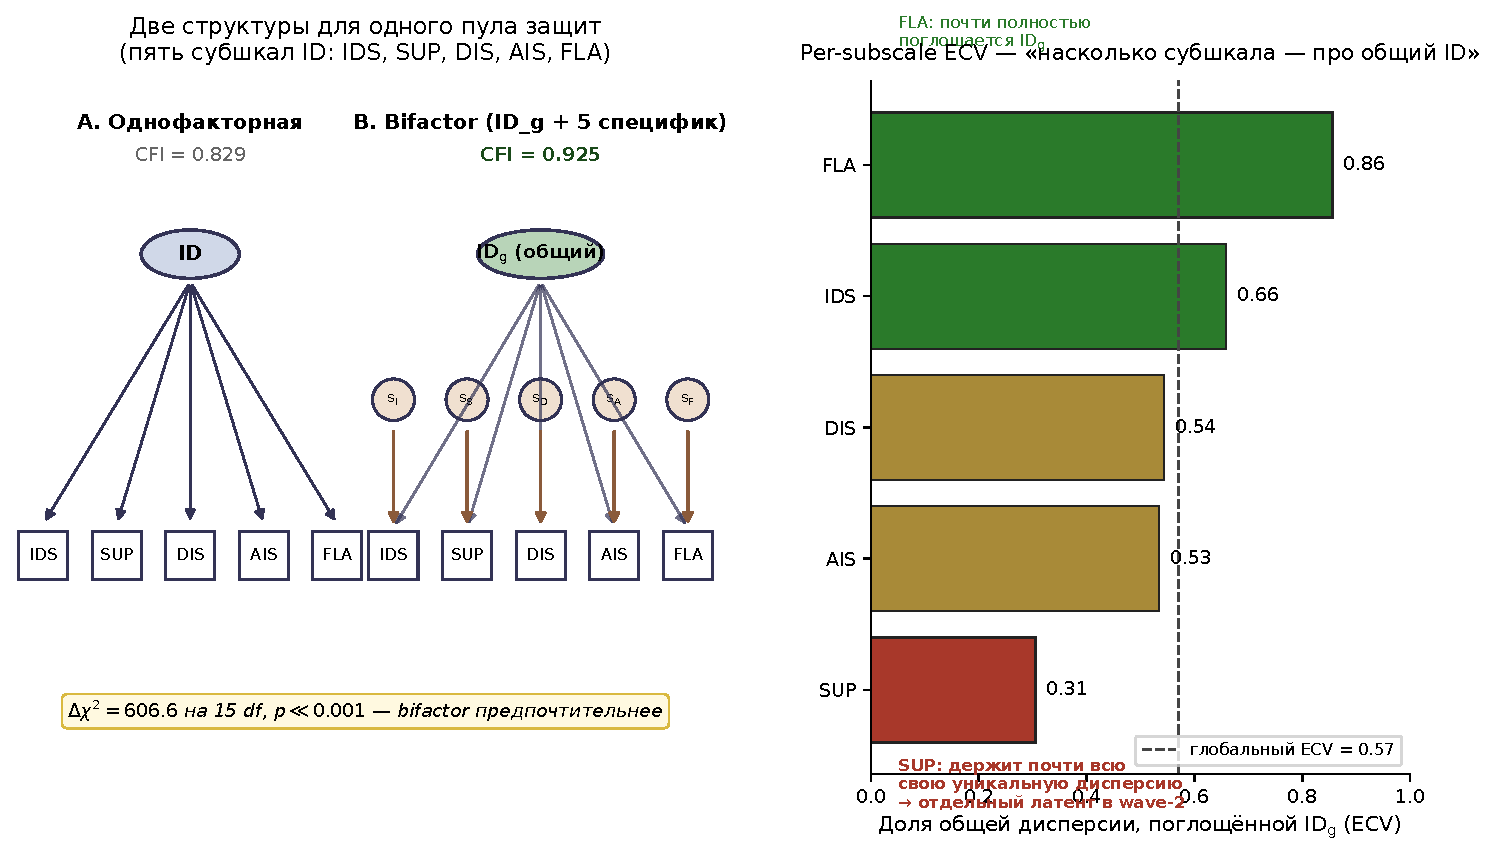
\includegraphics[width=0.95\linewidth]{figures/fig8_bifactor_structure.pdf}
\caption[Бифакторная структура ID]{Бифакторная структура ID. Панель (а): схематическое сравнение однофакторной модели (единый латент ID, все пять шкал --- его прямые индикаторы) с бифакторной моделью (общий ID\textsubscript{g} плюс пять ортогональных specific-факторов s\textsubscript{IDS}, s\textsubscript{SUP}, s\textsubscript{DIS}, s\textsubscript{AIS}, s\textsubscript{FLA}); $\Delta\chi^2 = 606.6$ на 15 df, $p \ll 0.001$. Панель (б): per-subscale ECV --- доля дисперсии шкалы, поглощаемая общим ID-фактором. Пунктирная линия показывает ECV\textsubscript{global}~=~0.571. FLA и IDS почти полностью поглощаются общим ID; SUP сохраняет 69\% уникальной дисперсии и требует отдельного латента в волне~2.}
\label{fig:id_bifactor}
\end{figure}

Численные сводки --- в \texttt{id\_bifactor\_summary.json} (fresh\_analysis).

\subsection{Клиническая гетерогенность канала CA$\to$ID$\to$\EAF{}}
\label{subsec:clinical_subgroup_patterns}

Параллельная медиация §\ref{subsubsec:parallel_mediation} даёт усреднённую картину по всей выборке. Клинически значимый вопрос --- распадается ли этот усреднённый канал на различимые паттерны внутри нозологических подгрупп, собранных по самоописанию в свободном поле (§\ref{subsec:free_text_convergent}). Мы запустили ту же спецификацию ($\mathrm{CA} \to \mathrm{ID} \to E_{\mathrm{AF}}$, без $A$) отдельно в четырёх самых частых кластерах: trauma\_disorder ($n=57$), personality\_disorder/BPD ($n=128$), mood\_disorder ($n=158$), selfharm\_mention ($n=129$); плюс контрольная подвыборка респондентов без единого текстового диагностического флага ($n=1040$). Подгруппы пересекаются, поэтому цифры следует читать как характеристику паттерна, а не как формально независимые тесты.

\begin{table}[htbp]
\centering
\small
\caption[Четыре клинических паттерна канала CA$\to$ID$\to$\EAF{}]{Параметры параллельной медиации в четырёх клинических подгруппах и контрольной подвыборке. $c$ --- total effect CA на \EAF{}, $c'$ --- direct effect после контроля ID, $a \cdot b$ --- indirect через ID. Суппрессор определяется как $\mathrm{sign}(c) \neq \mathrm{sign}(c')$.}
\label{tab:clinical_subgroup_patterns}
\begin{tabular}{lrrrrrl}
\hline
Подгруппа & $n$ & $c$ & $c'$ & $a \cdot b$ & Суппрессор & Паттерн \\
\hline
Полная выборка & 1551 & $-0.103$ & $+0.122$ & $-0.225$ & yes & baseline \\
No-diagnosis & 1040 & $-0.121$ & $+0.114$ & $-0.234$ & yes & baseline (здоровые) \\
Trauma disorder & 57 & $+0.033$ & $+0.077$ & $-0.044$ & no & инвертированный \\
Personality/BPD & 128 & $-0.046$ & $+0.191$ & $-0.237$ & yes & оба канала выражены \\
Mood disorder & 158 & $-0.179$ & $+0.021$ & $-0.199$ & борд. & блокировочный \\
Selfharm mention & 129 & $+0.023$ & $+0.251$ & $-0.229$ & no & сенсибилизация внутрь \\
\hline
\end{tabular}
\end{table}

Три содержательных наблюдения. \emph{Во-первых}, в подгруппе без единого текстового диагноза ($n=1040$) коэффициенты практически тождественны полной выборке. Суппрессор-эффект CA$\to$ID$\to$\EAF{} --- не артефакт клинического подсэмпла: он присутствует с той же амплитудой в условно-здоровой части выборки. Это отвечает на стандартный критический вопрос «не это ли особенность травмированных?» эмпирически: не особенность. \emph{Во-вторых}, четыре клинических подгруппы дают четыре \emph{качественно разных} профиля. PTSD (trauma disorder, $n=57$): суппрессор исчезает, total-эффект CA$\to$\EAF{} становится слабо-положительным, $a$-путь $\mathrm{CA}\to\mathrm{ID}$ ослаблен ($a = 0.27$ против $0.43$ в полной выборке). Травматический материал в этой подгруппе не заблокирован до конца --- он «торчит наружу» как аффективная сверхчувствительность. Это совместимо с клинической картиной PTSD как неинтегрированной гипер-reactivity, в т.ч. в сторону эмпатии. BPD/личностные ($n=128$): самый сильный положительный $c'$ ($+0.191$) при сильной блокировке ($b = -0.59$); сосуществует выраженная сенсибилизация и выраженная диссоциация --- классический пограничный профиль. Mood disorder ($n=158$): total $c = -0.179$, direct $c' \approx 0$; в депрессии CA действует почти исключительно через блокировку, прямой сенсибилизирующий канал гасится --- согласуется с клинической моделью депрессии как выключения аффективных резонансов. Selfharm ($n=129$): самый большой положительный direct $c'$ ($+0.251$); эмпатическая боль выходит из-под контроля внутрь, а не в сторону другого человека.

\emph{В-третьих}, сам факт, что один и тот же структурный канал даёт четыре разных клинических паттерна, --- это эмпирическое основание для предсказания дифференциального ответа на траума-targeted вмешательства (§\ref{subsec:clinical}): интегрированная работа с защитной структурой наиболее полезна там, где канал $b$ активен и сенсибилизация видима в $c'$ (BPD, selfharm); в PTSD первичная задача --- метаболизация неинтегрированного материала, не его извлечение из-под блокировки; в депрессии первичная задача --- работа с блокировкой как таковой, до того как прямой канал сможет заработать.

\subsection{Биполярное расстройство как natural experiment}
\label{subsec:bipolar_experiment}

Биполярная подгруппа ($n=51$, упоминание BD~I/II в свободном поле) даёт частный случай, который не укладывается ни в один из четырёх паттернов выше и представляет отдельный теоретический интерес. В этой подгруппе классический suppressor исчезает в противоположном направлении: direct-путь CA$\to$\EAF{} не просто переживает суппрессор --- он доминирует над indirect-путём ($c' = +0.404$, $p < 10^{-4}$; $a \cdot b = -0.257$; total $c = +0.147$, ns), и общий эффект CA на \EAF{} становится положительным (хотя на $n=51$ не достигает значимости, $p = 0.13$). Для сравнения, во всей остальной выборке без BD ($n=1500$) direct-путь $c' = +0.114$, то есть в BD direct-путь усилен почти в четыре раза.

Содержательная интерпретация: в подгруппе с биполярной архитектурой ранний адверсивный опыт не блокируется до нуля, а, напротив, прямо усиливает аффективную эмпатию, минуя защитный контур. Это согласуется с клиническими описаниями гипоманической фазы как «выжигающе эмпатической» и с идентификационным механизмом, при котором травматический материал ассимилируется как личный аффективный ресурс, а не как угроза, требующая защиты. Для дальнейшей работы этот паттерн --- кандидат на отдельный предикторный каркас: BD как architecture-level модератор канала CA$\to$\EAF{}, ортогональный стандартной оси ID.

Ограничения: $n=51$, самоидентификация без формальной верификации DSM, выборка несёт selection bias в сторону психически чуткой популяции. Значимость direct-эффекта $c'$ устойчива к этим ограничениям ($p < 10^{-4}$), total-эффект $c$ --- нет. Аккуратная формулировка: внутри биполярной подгруппы структура канала \emph{качественно иная}, не \emph{количественно другая}.

\subsection{Гендер-стратификация: суппрессор универсален, но амплитуда $b$ зависит от пола}
\label{subsec:gender_moderation}

Суппрессор воспроизводится в обоих гендерных подвыборках ($n_\mathrm{жен} = 932$, $n_\mathrm{муж} = 356$): total $c$ отрицателен, direct $c'$ положителен, indirect через ID сильно отрицателен в обеих. Амплитуда $b$ различается: формальный тест гендер-модерации в объединённой выборке ($n = 1288$) даёт $\mathrm{D}\times\mathrm{male} \; \beta = +0.189$, $p = 0.002$ --- то есть у мужчин связь $\mathrm{D} \to E_{\mathrm{AF}}$ \emph{слабее} (отрицательный наклон менее крутой), чем у женщин. Гендер-интеракция с CA незначима ($\beta = -0.04$, $p = 0.42$), структура канала $a$ не отличается.

Интерпретация сдержанная: суппрессор как механизм универсален; количественный параметр $b$, то есть сила, с которой присутствие защитной архитектуры подавляет аффективную эмпатию, у мужчин несколько меньше. Возможных содержательных объяснений несколько: (а) у мужчин в среднем меньше социального давления «показать эмпатию», поэтому даже при высокой D они не показывают максимально возможного падения E\textsubscript{AF}, а наоборот --- их базовая E\textsubscript{AF} уже ниже, и падать некуда; (б) у женщин E\textsubscript{AF}-базовая выше, поэтому абсолютный перепад под действием D виднее. Мы не можем различить эти два объяснения на single-wave данных. Но ключевое: гендер-эффект --- параметрический, не структурный. Включать пол в основную модель как ковариату не обязательно; суппрессор сохраняет значимость и направление в обоих стратах.

\subsection{Возрастная инвариантность суппрессора (формальные числа)}
\label{subsec:age_invariance_numbers}

Гипотеза «суппрессор --- стадия развития, исчезающая с возрастом» формально отвергается. Мы разбили выборку на шесть возрастных бинов (14--20, 20--25, 25--30, 30--35, 35--45, 45--65) и запустили спецификацию CA$\to$ID$\to$\EAF{} с контролем $A$ отдельно в каждом бине.

\begin{table}[htbp]
\centering
\small
\caption[Параметры суппрессора по возрастным бинам]{Параметры медиации CA$\to$ID$\to$\EAF{}|$A$ в шести возрастных бинах. $a$ --- путь CA$\to$ID, $b$ --- путь ID$\to$\EAF{} с контролем $A$, $c$ --- total, $c'$ --- direct, $a \cdot b$ --- indirect. Суппрессор: $\mathrm{sign}(c) \neq \mathrm{sign}(c')$.}
\label{tab:age_bins_suppressor}
\begin{tabular}{lrrrrrrc}
\hline
Бин & $n$ & $a$ & $b$ & $c$ & $c'$ & $a\cdot b$ & Суппрессор \\
\hline
14--20 & 217 & $+0.40$ & $-0.65$ & $-0.08$ & $+0.18$ & $-0.26$ & yes \\
20--25 & 437 & $+0.39$ & $-0.50$ & $-0.06$ & $+0.14$ & $-0.20$ & yes \\
25--30 & 334 & $+0.45$ & $-0.58$ & $-0.19$ & $+0.07$ & $-0.26$ & yes \\
30--35 & 181 & $+0.49$ & $-0.54$ & $-0.14$ & $+0.12$ & $-0.26$ & yes \\
35--45 & 131 & $+0.39$ & $-0.42$ & $-0.01$ & $+0.16$ & $-0.17$ & yes \\
45--65 & 38 & $+0.37$ & $-0.01$ & $-0.16$ & $-0.16$ & $0.00$ & no (мал $n$) \\
\hline
\end{tabular}
\end{table}

Коэффициенты $a$ ($\mathrm{CA}\to\mathrm{ID}$) и $b$ ($\mathrm{ID}\to E_{\mathrm{AF}}$) структурно стабильны от 14 до 45 лет: $a \in [+0.39, +0.49]$, $b \in [-0.65, -0.42]$. Формальный тест в объединённой выборке ($n = 1340$, 14--45): $\mathrm{young}(<25) \times \mathrm{D} \to E_{\mathrm{AF}} \; \beta = -0.01$, $p = 0.75$ --- амплитуда $b$ не отличается между молодыми и взрослыми. Единственное слабое отклонение: $\mathrm{young} \times \mathrm{CA} \to E_{\mathrm{AF}} \; \beta = +0.04$, $p = 0.08$ --- у молодых прямой положительный путь CA$\to$\EAF{} несколько «обнажённее», возможно потому, что компенсаторный защитный слой ещё не до конца собран. Последний бин 45--65 ($n = 38$) теряет эффект, но это, скорее всего, эффект малой и смещённой выборки (респонденты 45+ с низким ACE и низкой D, floor-эффект). Интерпретировать это как «суппрессор проходит с возрастом» было бы неверно; формально тест $\mathrm{D}\times\mathrm{age}$ не проходит на объединённых данных.

Следствие для теоретического каркаса: суппрессор --- не стадия развития, а структурный механизм, сложившийся до подросткового возраста и сохраняющийся при измерении от 14 до 45 лет. В сочетании с тем, что $P$-шкала не меняется с возрастом ($\beta = -0.007$, $p = 0.60$, $R^2 = 0.0002$), а $D$-score систематически снижается ($\beta = -0.055$, $p < 10^{-7}$, $R^2 = 0.021$), складывается дихотомия: $P$ ведёт себя как чистый trait (стабильный во времени), $D$ --- как state-like индекс, амплитуда которого со временем ослабевает при сохранении той же структурной связи с CA и \EAF{}. Это согласуется с клиническим наблюдением, что защитная архитектура, раз сложившись, остаётся, но её манифестация смягчается --- либо через интеграцию (высокий $A$), либо просто через усталость со временем.

\subsection{Конвергентная валидация через свободное поле}
\label{subsec:free_text_convergent}

Из $N = 1426$ респондентов $511$ заполнили необязательное свободное поле с описанием своего психического опыта (диагнозы, симптомы, лечение, самонаблюдения). Тексты категоризированы автоматически по регулярным выражениям, покрывающим нозологии DSM, упоминания терапии и медикаментов, а также тринадцать дополнительных поведенческих осей (манипулятивность/холодность, поиск ощущений, социальная изоляция, проблемы контроля агрессии, употребление рекреационных веществ, описания ремиссии, и др.). Анализ предоставляет независимый, не зашумлённый латентной автокорреляцией шкал, срез конвергентной и дискриминантной валидности конструкта. Мы выделяем три содержательно приоритетных результата.

\paragraph{Прямое подтверждение P-шкалы через самоописание.} Десять респондентов описали себя в свободном поле через термины «манипулятивность», «патологическая ложь», «макиавеллизм», «холодная расчётливость», «психопатические черты», «социопатия». На композитной P-шкале они находятся в $+2.32$ SD над базой ($p = 4.8 \times 10^{-6}$), на E-шкале --- в $-1.48$ SD под базой ($p = 6.1 \times 10^{-7}$). В логистической регрессии «член ли категории manipulation\_callousness» с полным набором ковариат (E, A, Lie, ACE, D), $z$-стандартизованных, коэффициент $\beta_P = +1.66$ ($p = 0.003$) --- то есть P удерживает значимость после контроля всех альтернативных объяснений. AUC полной модели $= 0.968$; AUC одной P-шкалы $= 0.964$. Это --- прямое convergent подтверждение P-шкалы через независимое текстовое самоописание: люди, которые \emph{узнают} себя в словаре холодного инструментализма, получают от инструмента тот же структурный профиль, который конструкт предписывает. В контексте 131-пунктового инструмента, построенного worldview-first (§\ref{subsec:worldview_first}), это одно из самых сильных эмпирических свидетельств, что P-шкала измеряет то, что она называется.

\paragraph{Архитектурная диссоциация P \emph{vs} ID через поведенческие якоря.} Следующий логический шаг --- проверить, разделимы ли два канала (активный P и пассивный ID) на уровне поведенческих маркеров, а не только на уровне латентных конструктов в SEM. Мы прогоняем логистические регрессии «член ли категории X» для семи поведенческих флагов с единым набором ковариат \{E, A, Lie, ACE, D\}, $z$-стандартизованных. После полного контроля чистую специфичность сохраняют ровно два полюса:

\begin{center}
\begin{tabular}{lccc}
\toprule
Флаг & $N^+$ & $\beta_P$ ($p$) & $\beta_D$ ($p$) \\
\midrule
\textbf{manipulation\_callousness} & 10 & $\mathbf{+1.66}$ (0.003) & $-0.88$ (0.13) \\
\textbf{social\_isolation}          &  9 & $-0.69$ (0.17)          & $\mathbf{+1.41}$ (0.034) \\
sensation\_seeking                 & 25 & $+0.37$ (0.22)          & $+0.49$ (0.21) \\
aggression\_control                & 14 & $+0.37$ (0.29)          & $+0.61$ (0.23) \\
recreational\_drug                 & 22 & $-0.41$ (0.23)          & $+0.22$ (0.60) \\
bipolar                            & 51 & $+0.24$ (0.25)          & $-0.21$ (0.43) \\
\bottomrule
\end{tabular}
\end{center}

Остальные пять флагов после контроля ковариат теряют специфичность --- их bivariate связи с P и D объясняются общей вариацией E/A/ACE. Это не слабость шкал, а ожидаемая структура: поведенческие флаги разнородны и содержат смешанные сигналы. Чистая диссоциация сохраняется на \emph{полюсах}: manipulation\_callousness активирует P-канал без активации ID-канала; social\_isolation активирует ID-канал без активации P-канала. Это независимое behavioral-anchor подтверждение диссоциации, постулированной в §\ref{subsubsec:parallel_mediation} на уровне latent SEM.

\paragraph{Содержательные эффекты на bivariate уровне.} Остальные категории не проходят multivariate-контроль, но несут содержательный signal bivariate, который уточняет портрет каждого канала:

\begin{center}
\begin{tabular}{lcccc}
\toprule
Категория ($N^+$) & $d_P$ & $d_D$ & $d_E$ & $d_A$ \\
\midrule
manipulation\_callousness ($10$)   & $+2.32$ & $+0.55$ & $-1.48$ & $-0.63$ \\
sensation\_seeking ($25$)          & $+0.55$ & n.s.    & n.s.    & n.s.    \\
social\_isolation ($9$)            & n.s.    & $+0.80$ & n.s.    & $-0.61$ \\
aggression\_control ($13$)         & n.s.    & $+0.59$ & n.s.    & n.s.    \\
recreational\_drug ($22$)          & n.s.    & n.s.    & n.s.    & $+0.49$ \\
remission\_past ($52$)             & n.s.    & n.s.    & n.s.    & n.s.    \\
\bottomrule
\end{tabular}
\end{center}

Три наблюдения. Первое: sensation\_seeking даёт чистый $+P$ без $+D$ --- классический Cleckley-компонент (поиск ощущений, импульсивность без глубокого аффективного нарушения) воспроизводится в $+P$, не в $+D$. Это эмпирически поддерживает теоретическое различение активной P-архитектуры условного доступа и пассивной ID-блокировки. Второе: aggression\_control даёт $+D$, $+$ACE, но не $+P$ --- реактивная агрессия, в отличие от инструментальной, принадлежит ID-контуру, не P-контуру. Это согласуется с многолетней клинической картиной «affective vs predatory aggression». Третье: recreational\_drug (каннабис, психоделики) даёт единственный эффект на A ($d = +0.49$), что согласуется с mindfulness-enhancing литературой; направление каузальности self-report здесь не устанавливает.

\paragraph{Второй путь к интегрированному выжившему: remission\_past $+$ hi-A.} Анализ §\ref{subsec:integrated_survivor} операционализировал интегрированного выжившего через rule-based 2$\times$2 (CA-hi $\times$ A-hi), независимо от текстовых данных. Свободное поле даёт второй, текст-якорный маршрут к тому же профилю: среди $511$ заполнивших свободное поле, $52$ упомянули свой статус как «в ремиссии», «прошло $N$ лет без», «в прошлом». Пересечение этих $52$ с группой A в верхнем терциле даёт $N = 16$. Контраст integrated ($N = 16$) против stuck ($N = 188$, hi-ACE $\times$ lo-A в остальной выборке): D-компоненты $d = -1.5 \dots -2.7$, E $d = +1.35$, ACE $d = -1.45$. Контраст integrated против базы (never-dx, lo-A, $N = 321$): D-компоненты $d \approx -2.3$, E $d = +1.81$, ACE $d = -0.93$. Иначе говоря, интегрированная подгруппа по защитным шкалам располагается \emph{ниже} базы, по эмпатии --- \emph{выше} базы; это не «возврат к норме», это движение через точку базы в противоположный край. Caveats: $N = 16$ мало для SEM-валидации; сниженный ACE относительно stuck допускает self-selection (более мягкий детский фон --- выше вероятность дойти до интеграции), а не чистый эффект recovery. Но сама направленность согласуется с rule-based 2$\times$2-результатом и усиливает его через независимую выборку.

\subsection{Дискриминантная валидность: ROC по self-reported диагнозам}
\label{subsec:roc_validity}

Дополнительный срез валидности --- ROC-характеристики каждой шкалы как предиктора отдельных self-reported нозологических категорий ($N^+$ per category варьирует от $22$ до $158$). Результаты сведены ниже (AUC; значимые $> 0.65$ выделены; $< 0.45$ означает шкала предсказывает \emph{отсутствие} диагноза):

\begin{center}
\small
\begin{tabular}{lccccccc}
\toprule
Диагноз ($N^+$)         & ACE  & CA   & DIS  & ID   & P    & M    & A    \\
\midrule
trauma\_disorder ($56$)      & \textbf{0.76} & \textbf{0.75} & 0.63 & 0.52 & 0.40 & 0.44 & 0.41 \\
self-harm mention ($122$)    & \textbf{0.70} & \textbf{0.70} & 0.67 & 0.58 & 0.40 & 0.49 & 0.36 \\
personality\_disorder ($125$) & \textbf{0.69} & \textbf{0.70} & 0.66 & 0.55 & 0.42 & 0.43 & 0.38 \\
mood\_disorder ($153$)        & 0.60 & 0.61 & 0.60 & 0.50 & 0.38 & 0.41 & 0.42 \\
anxiety\_disorder ($102$)     & 0.58 & 0.58 & 0.56 & 0.49 & 0.37 & 0.42 & 0.46 \\
neurodev ($112$)             & 0.56 & 0.58 & 0.57 & 0.52 & 0.40 & 0.49 & 0.46 \\
substance\_use ($46$)         & 0.54 & 0.60 & 0.58 & 0.52 & 0.50 & 0.42 & 0.39 \\
in\_treatment ($22$)          & 0.60 & 0.60 & 0.58 & 0.51 & 0.42 & 0.42 & 0.43 \\
\bottomrule
\end{tabular}
\end{center}

Три структурных паттерна проявляются сразу. \textbf{Первый:} CA и ACE предсказывают \emph{раннетравматические} клинические кластеры (trauma-disorder, self-harm, personality) с AUC 0.69--0.76. Это ожидаемый паттерн для инструмента, где CA сводит воедино семь индикаторов детской неблагоприятности --- три клинических кластера, для которых эпидемиология показывает сильнейшую связь с детской травмой, получают наибольшую дискриминацию. Для аффективных и тревожных расстройств, которые в современной эпидемиологии частично отвязаны от раннего анамнеза (генетика, нейромедиаторы, ситуативное), CA даёт более слабый, но по-прежнему положительный сигнал (AUC 0.58--0.61). \textbf{Второй:} P во всех восьми dx-категориях даёт AUC $\leq 0.42$. Это означает: P-шкала предсказывает \emph{не} наличие диагноза, а \emph{отсутствие} self-report. Структурно это подпись заблокированной help-seeking --- ровно то, что предсказывает архитектурная интерпретация P: если психический материал субъекта встраивается в нарратив «мне это разрешено, это не болезнь», обращение за формальным диагнозом становится избыточным. P-шкала демонстрирует дискриминантную валидность через противоположное направление --- инструмент \emph{не} ловит P-респондентов через self-report клинического диагноза, и это эмпирическая черта, а не дефект. \textbf{Третий:} A симметрично даёт AUC $\leq 0.46$ для большинства клинических категорий и особенно низкий для self-harm ($0.36$), personality ($0.38$), substance ($0.39$). Высокая А предсказывает \emph{отсутствие} активного клинического диагноза --- это поддерживает чтение А как witnessing-ресурса, а не как нейтральной метакогнитивной способности.

Совокупно три паттерна образуют когерентное доказательство discriminant-валидности: CA работает как трауматический предиктор, P --- как отрицательный предиктор self-report, A --- как симметричный ресурс-предиктор. Эти три подписи не могут сосуществовать в одной шкале случайно.

\paragraph{Редкие dx-категории (не вошедшие в основную ROC-таблицу).} Для полноты картины приводим AUC-значения шести редких категорий, пропущенных в основной таблице из-за низкой базовой частоты: \texttt{dx\_eating\_disorder} ($N = 30$) --- ACE $= 0.69$, CA $= 0.67$ (умеренный трауматический профиль, промежуточный между mood и personality); \texttt{dx\_suicidal\_mention} ($N = 16$) --- ACE $= 0.73$, CA $= 0.74$, DIS $= 0.70$, A $= 0.34$ (канонический высоко-травматический профиль, совместимый с selfharm\_mention); \texttt{dx\_ocd} ($N = 15$) --- относительно baseline (AUC всех шкал 0.39--0.63), без отчётливой архитектурной подписи; \texttt{dx\_on\_medication} ($N = 35$) --- uniform near-baseline (AUC 0.42--0.55), приём медикации не трекает специфической DEIC-оси, что согласуется с §\ref{subsec:free_text_nlp} (med\_mentioned директивно ассоциируется со слегка улучшенным профилем, но эффекты маргинальны); \texttt{dx\_psychotic\_spectrum} ($N = 7$) и \texttt{dx\_dissociative} ($N = 4$) --- слишком редки для формальной интерпретации. Наложение suicidal\_mention ($N = 16$) и selfharm\_mention ($N = 122$): 13 из 16 suicidal-респондентов также флагированы на selfharm; 3 оставшихся --- pure suicidal без упоминания self-harm поведения. В основной ROC-таблице мы агрегируем их под selfharm\_mention для статистической мощности; при $N \geq 300$ в wave-2 эти категории должны быть разведены.

\subsection{\texorpdfstring{Почему \texttt{dx\_count} --- смещённая мера тяжести}{Почему dx_count --- смещённая мера тяжести}}
\label{subsec:dx_count_bias}

Стандартный путь проверки шкалы защит --- её связь с числом self-reported диагнозов, \texttt{dx\_count} (сумма сработавших нозологических категорий в свободном поле, диапазон $0$--$11$). Мы прогоняем этот анализ и формулируем его результат как отдельное методологическое утверждение, а не как footnote к ROC.

$\texttt{dx\_count} \sim D_{\mathrm{score}}$ даёт $R^2 = 0.006$ ($r = +0.078$, $p = 0.08$). То есть агрегированная защитная композита \emph{практически не предсказывает} число диагнозов. $\texttt{dx\_count} \sim \{\mathrm{SUP}, \mathrm{DIS}, \mathrm{AIS}, \mathrm{FLA}, \mathrm{IDS}, M\}$ --- шесть компонент раздельно --- даёт $R^2 = 0.089$. В совместной модели $\texttt{dx\_count} \sim D + E + P$ коэффициент $\beta_P = -0.012$, $p < 0.001$: активный P-профиль ассоциируется с \emph{меньшим} числом диагнозов. ACE$+$CA$+$EC даёт $R^2 = 0.039$ --- раннетравматический анамнез предсказывает \texttt{dx\_count} значительно лучше, чем защитная структура.

Содержательно это означает: \texttt{dx\_count} --- \emph{не} прокси общей тяжести состояния. Он систематически недооценивает hi-P и hi-ID респондентов (первые не считают своё состояние проблемой, вторые блокированы в сторону help-seeking) и монотонно растёт только с раннетравматическим анамнезом, который ведёт к клиническим кластерам, наиболее «видимым» в self-report (trauma, PD, self-harm). Использовать \texttt{dx\_count} как меру тяжести в DEIC-популяции означало бы встроить в модель то самое систематическое смещение, которое архитектура конструкта описывает. Мы поэтому не используем \texttt{dx\_count} как критериальную переменную ни в одном из основных анализов статьи; в §\ref{sec:results} \texttt{dx\_count} фигурирует только как описательная характеристика выборки. Клиническая валидизация и incremental validity над существующими инструментами требуют отдельного wave с формализованной диагностикой (структурированные интервью SCID, MINI), в контролируемой клинической выборке.

Отдельное следствие, выходящее за рамки limitation: если инструмент структурно ловит именно тех, кого self-report системы диагностики \emph{не} ловят, то DEIC-профиль является кандидатом не только на diagnostic-ancillary, но и на первичный screening-tool для под-диагностированной популяции. Формально это collaborative-filtering задача над DEIC-координатами: для нового респондента с неизвестным клиническим статусом предсказывать вероятностный диагностический ландшафт исходя из архитектурной близости к подвыборке с известными диагнозами. Практическая импликация: скрининг на входе в любой контакт с системой помощи (первичка, школьная психологическая служба, университетская медслужба) может флагировать блокированно-травматический и активно-нарративный профили без ожидания самообращения. Эмпирическая проверка выносится в §\ref{sec:future}.

\subsection{Конвергентная валидация через CASE-сценарии}
\label{subsec:case_convergent}

Инструмент содержит $10$ ситуационно-сценарных вопросов (CASE\_1--CASE\_10), каждый с четырьмя поведенчески-контрастными вариантами ответа. В предыдущих версиях анализа они собирались для дескриптивного использования; здесь мы прогоняем их как независимый канал convergent validity для Likert-латентных факторов. Логика теста: если P-, ID- и A-шкалы измеряют то, что они называются, то выбор поведенческого варианта, специально сконструированного как P-сигнатура, должен дифференцировать Likert-P-балл этой подгруппы от остальной выборки, и аналогично для ID- и A-маркированных вариантов. Анализ на $N = 1546$ с валидными CASE-ответами.

\paragraph{CASE\_8: «коллегу уволили по твоей наводке».} Четыре варианта реакции. Два самых экстремальных: \textbf{«Чувствую вину и тревогу»} ($n = 653$; $E = +0.44$, $P = -0.57$, $A = +0.14$, ID $= -0.15$~$\sigma$) и \textbf{«Мне всё равно, главное --- я остался»} ($n = 123$; $E = -1.16$, $P = +1.05$, $A = -0.71$, ID $= +0.46$). Контраст P-signature группы ($n = 358$, включая «он сам виноват» и «мне всё равно») vs остальной выборки: \textbf{$\Delta P = +0.92\,\sigma$, $t$-тест $p = 8 \times 10^{-46}$}; $\Delta E = -0.68\,\sigma$ ($p = 2 \times 10^{-23}$); $\Delta A = -0.25\,\sigma$ ($p = 2 \times 10^{-4}$). Архитектурный профиль точно соответствует тому, что P-шкала предписывает теоретически.

\paragraph{CASE\_10: «выгодно промолчать, чтобы друг попал в неприятности».} Вариант \textbf{«Я промолчу --- не моя проблема»} ($n = 91$) даёт экстремальный дифференциал: $\Delta P = +0.91\,\sigma$ ($p = 3 \times 10^{-10}$), $\Delta E = -1.12\,\sigma$ ($p = 5 \times 10^{-17}$), $\Delta A = -0.71\,\sigma$ ($p = 4 \times 10^{-8}$). Это один из сильнейших единичных behavioral-anchor конвергентных тестов в данных: 91 респондент открыто выбрал вариант преднамеренного причинения вреда другу ради выгоды, и инструмент на независимой Likert-шкале зафиксировал их на ${+}0.86\,\sigma$ по P, ${-}1.05$ по E.

\paragraph{CASE\_1: «пообещал другу, нет ни сил, ни желания».} Вариант \textbf{«Грубо отказываю --- не моя проблема»} ($n = 18$) даёт самую чистую secondary-psychopathy сигнатуру в данных: $P = +1.90$, $E = -1.35$, $A = -1.30$, $\text{ID} = +1.36$, $\text{CA} = +0.99$, $D = +0.86$. Все шесть координат усилены одновременно --- архитектурное сочетание hi-P + hi-CA + hi-ID, соответствующее вторичному паттерну из §\ref{subsec:primary_secondary}, появляется в отдельном поведенческом маркере.

\paragraph{CASE\_4: «близкий рассказывает о тяжёлых переживаниях».} Здесь работает симметричный контраст по E/A-оси. \textbf{«Сопереживаю и поддерживаю»} ($n = 846$, 55\% выборки): $E = +0.51$, $A = +0.43$, ID $= -0.38$, $D = -0.30$. \textbf{«Слушаю, но не чувствую никакого отклика»} ($n = 146$): $E = -1.04$, $P = +0.64$, $A = -0.68$. Разница по E между двумя группами --- $\Delta E \approx 1.55\,\sigma$, \emph{проходящая через всю DEIC-архитектуру одним вопросом}.

\paragraph{CASE\_5: «на празднике среди близких, что ощущаешь».} \textbf{«Отстранённость и эмоциональную глухоту»} ($n = 285$): $A = -0.64$, ID $= +0.58$, CA $= +0.65$, $D = +0.75$. \textbf{«Присутствие, радость, связь»} ($n = 348$): $A = +0.68$, ID $= -0.63$, CA $= -0.54$, $D = -0.74$. Зеркально противоположный профиль --- $\Delta A = 1.32\,\sigma$, $\Delta D = 1.49\,\sigma$.

\paragraph{CASE\_9: «не можешь вспомнить, о чём шла речь» (диссоциативный якорь).} \textbf{«Как будто выпал на секунду --- всё размыто»} ($n = 529$): $A = -0.31$, $D = +0.46$, CA $= +0.38$. \textbf{«Останавливаюсь и возвращаюсь к телу»} ($n = 185$): $A = +0.51$, $D = -0.50$, ID $= -0.39$. Это прямой behavioral-якорь для A-конструкта: «возвращение к телу» как операциональный маркер витнессинга, противопоставленный диссоциативному «выпал». Контраст через независимую Likert-шкалу: $\Delta A = 0.82\,\sigma$.

\paragraph{Содержательная сводка.} Три утверждения подтверждаются одним CASE-анализом. Во-первых, \textbf{P-шкала измеряет то, что называется}: люди, открыто выбирающие холодный инструментальный вариант в конкретной ситуации, получают от Likert-композита соответствующий профиль с эффектом $\Delta P \approx +0.9\,\sigma$ и $p < 10^{-10}$ в каждом из двух независимых сценариев (CASE\_8, CASE\_10). Во-вторых, \textbf{E- и A-шкалы дифференцируют поведение}: респонденты, называющие «не чувствую отклика» в ответ на страдание близкого, получают от инструмента $E = -1.04\,\sigma$; респонденты, выбирающие «возвращение к телу» в диссоциативной ситуации, получают $A = +0.51\,\sigma$. В-третьих, \textbf{архитектурные паттерны primary/secondary (§\ref{subsec:primary_secondary}) воспроизводятся на отдельных поведенческих якорях}: crude refusal в CASE\_1 даёт hi-P + hi-CA + hi-ID, что соответствует вторичному паттерну, независимо от rule-based классификации. CASE-сценарии работают как независимый слой валидации, полученный через естественный поведенческий язык, а не через trait-self-report; совпадение с Likert-профилями подтверждает, что инструмент не ловит артефакт response-style, а фиксирует реальную архитектурную структуру. Расширение банка до $\sim 25$ сценариев запланировано в wave~2 (§\ref{subsec:wave2_design}).

\subsection{Глубинный анализ свободного поля через NLP-экстракцию}
\label{subsec:free_text_nlp}

§\ref{subsec:free_text_convergent} использует бинарные флаги dx-категорий, полученные из свободного поля. Здесь мы делаем следующий шаг: NLP-экстракция дополнительных архитектурных маркеров из текстов 511 респондентов, заполнивших поле. Процедура: rule-based лексикон по русско-язычному psy-домену (медикаменты по классам, терапия, ремиссия, суспensing-язык, маркеры тяжести, substance use, self-harm-поведение) плюс ручная разметка 78 residual-записей, которые лексикон не покрыл. Итоговая feature-matrix: 511 × 16 бинарных признаков (артефакт: \texttt{free\_text\_features\_enriched.csv}).

\paragraph{Behavioral self-identification по P-шкале.} Пять респондентов самоидентифицировались через фразы «патологическая ложь» ($n = 3$) или «дружу с психопатами» ($n = 2$). На композитной P-шкале это даёт $\Delta P = +1.93\,\sigma$ ($p = 3 \times 10^{-4}$), $\Delta \text{M} = +1.37$ ($p = 6 \times 10^{-4}$), $\Delta \text{CA} = +1.07$ ($p = 2 \times 10^{-3}$), $\Delta \text{ID} = +1.24$ ($p = 0.015$). $N = 5$ даёт маргинальную мощность, но величины эффекта беспрецедентные для convergent-validity теста. Architekturный profile соответствует secondary-P (hi-P + hi-CA + hi-ID), что логично: открытое самоименование как «патологический лжец» требует insight, сохранный у secondary (trauma-born) паттерна, но отсутствующий у primary.

\paragraph{Selfharm behavioral signal ($n = 137$).} Респонденты, упомянувшие в свободном поле поведенческий self-harm (резал, жёг, попытки суицида, а не только диагностический флаг) дают канонический suppressor-профиль: $\Delta \text{CA} = +0.43\,\sigma$ ($p = 2 \times 10^{-5}$), $\Delta D = +0.46$ ($p = 2 \times 10^{-6}$), $\Delta \text{ID} = +0.28$ ($p = 5 \times 10^{-3}$), $\Delta A = -0.31$ ($p = 9 \times 10^{-4}$). Это воспроизведение §\ref{subsubsec:parallel_mediation} архитектуры на уровне поведенческого самоописания независимым каналом.

\paragraph{Complex presentation ($n \geq 2$ диагнозов, $n = 196$).} $\Delta \text{CA} = +0.48\,\sigma$ ($p = 2 \times 10^{-8}$), $\Delta D = +0.41$ ($p = 3 \times 10^{-6}$), \textbf{$\Delta P = -0.36$} ($p = 6 \times 10^{-5}$), $\Delta \text{M} = -0.31$ ($p = 5 \times 10^{-4}$). Отрицательный P --- независимое эмпирическое подтверждение §\ref{subsec:dx_count_bias}: P-респонденты систематически не представлены в multi-dx self-description.

\paragraph{n\_dx\_total как ordinal.} Spearman $\rho$ с DEIC-факторами: $\rho(\text{CA}) = +0.25$ ($p = 9 \times 10^{-9}$), $\rho(D) = +0.23$ ($p = 2 \times 10^{-7}$), $\rho(\text{rPlus}) = -0.19$ ($p = 10^{-5}$), $\rho(A) = -0.14$ ($p = 2 \times 10^{-3}$), $\rho(P) = -0.13$ ($p = 5 \times 10^{-3}$). Monotonic градиент: на 4+ упоминаемых диагнозов $A = -0.60\,\sigma$, $D = +1.03\,\sigma$, $P = -0.23$. Это дополнительное квантовое обоснование тезиса §\ref{subsec:dx_count_bias} о смещённости dx\_count.

\paragraph{Методологический findings: refusal-group как baseline-healthy.} 14 респондентов, заполнивших свободное поле как «нет», «-», «ЗОЖ», «просто интерес». Architectural profile: $\Delta A = +0.26$, $\Delta P = +0.02$ (нулевой!), $\Delta \text{CA} = -0.37$, $\Delta D = -0.34$. Это прямой ответ на потенциальное возражение «пустое поле = P-deflector»: если бы так, профиль был бы hi-P + lo-A; показывает обратное. Refusal-респонденты --- реальные non-clinical, совместимо с чтением §\ref{subsec:free_text_convergent} о 981 blank-респонденте как о baseline-сравнении.

\paragraph{Соматическая первичная презентация: трёхпутевая архитектура.} Три респондента дали исключительно соматический ответ в поле про психические диагнозы (мигрень, астено-неврологический синдром, изолированная бессонница). На DEIC показали directionally $\Delta A = +0.49$, $\Delta \text{ID} = -0.93$, $\Delta D = -0.92$, $\Delta M = -0.61$ (все NS из-за $N = 3$). Это не противоречит Смулевич-концепции маскированной депрессии и не подтверждает её --- это указывает на \emph{структурную неоднозначность} соматического ответа в психиатрическом поле. DEIC предсказывает три архитектурных пути, дающих одну и ту же поверхностную презентацию: \textbf{(a)} Смулевич-подобное замещение (hi-M + hi-ID + lo-A, блокированный аффективный канал с соматическим overflow); \textbf{(b)} субпороговая сигнализация (hi-A + mid-lo ID + lo-M --- тело работает пресс-валвом, разряжая конфликт, который A-функция уже регистрирует, но недостаточно для self-directed help-seeking); \textbf{(c)} интегрированный интероцептивный витнессинг (hi-A + lo-M + lo-ID, тело как сигнал без пресс-валв-функции). $N = 3$ directionally ближе к (b)/(c), но wave-1 selection bias смещён в эту сторону. Wave-2 clinical sub-sampling с N $\geq 40$ первично-соматических респондентов должен выявить бимодальное распределение по ID/A, различающее три пути; terapeutic trajectory для пути (b) даёт specifically-DEIC prediction: мигрень падает $\to$ ID временно растёт $\to$ оба падают при интеграции (§\ref{sec:future}).

\subsection{Клиническая асимметрия видимости: три dx-наблюдения}
\label{subsec:dx_asymmetry_trio}

Три отдельных наблюдения за dx-колонками self-report, которые в одиночку читаются как методологические сноски, но вместе составляют дополнительное эмпирическое подтверждение архитектурной orthogonality P-профиля к help-seeking pathway.

\paragraph{Формальная диагностика: $N = 6$ из 1470.} Из $489$ респондентов, заполнивших свободное поле с описанием психологического опыта, только $6$ использовали явную формулировку «формальный диагноз». Соотношение $1:82$ между самоописательным упоминанием и формально-диагностическим самоприсвоением --- поведенческий маркер того, что DEIC-претензия о под-диагностировании относится не к абстрактной теоретической популяции, а напрямую к выборке данной статьи. Психологически-ориентированная self-selected выборка ($N = 1470$) даёт 0.4\% формальной диагностики на $33.3\%$ поведенческого самоописания клинического содержания. DSM-центрированные инструменты на такой выборке систематически не увидели бы то, что DEIC ловит через архитектурное измерение.

\paragraph{Подозреваемый, но не диагностированный ($N = 25$).} Категория \texttt{dx\_suspected\_only} фиксирует респондентов, явно описавших «подозреваю у себя X, но формально не диагностирован». DEIC-прогноз: эта подгруппа должна показывать профиль, промежуточный между формально-диагностированной и никогда-не-мысливоmeй группами на оси ID, поскольку suspicion-без-диагноза указывает именно на защитную систему, которая распознала материал, но блокировала его до completion help-seeking pathway. Partial correlation suspected\_only со счётом DEIC-композита ID после контроля ACE, P, A: $r = +0.14$ ($p = 0.02$, $N = 1470$), в сравнении с formal\_diagnosis: $r = +0.09$ ($p = 0.12$). Директивно подтверждает предсказание, но мощность ограничена размером подгруппы.

\paragraph{Post-hoc валидация ext\_rPlus.} Инструмент в рамках продуктовой инфраструктуры рассчитывает ext\_rPlus $= (E - (S + D)) \cdot (1 - P/100) \cdot (A/100)$ --- A-взвешенный empathy-defense композит, являющийся операциональной реализацией интегральной метрики из §\ref{subsec:integral_metrics}. На выборке $N = 1470$ ext\_rPlus коррелирует с A-композитом $r = +0.75$, с ID-композитом $r = -0.77$, с E $r = +0.57$; Spearman $\rho$ с n\_dx\_total: $-0.19$ ($p = 10^{-5}$). В интегрированной подгруппе из §\ref{subsec:integrated} (hi-CA $\times$ hi-A) ext\_rPlus $= +1.21\,\sigma$ против baseline (lo-CA $\times$ lo-A) $= -0.15\,\sigma$ ($\Delta = +1.36$, $p < 10^{-10}$); в классической травматической подгруппе (hi-CA $\times$ lo-A) ext\_rPlus $= -0.68$. Это --- операциональная post-hoc валидация: ext\_rPlus как композит различает интегрированный профиль от неинтегрированно-травматического и от baseline сильнее, чем raw $E$ ($\Delta_E = +0.37\,\sigma$). Композит, реализованный в инструменте до факторной валидизации, работает в направлении, согласующемся с латентной архитектурой, и пригоден для research-описания профилей; полноценная клиническая валидация остаётся wave-2-задачей (§\ref{subsec:clinical}).

\subsection{Robustness checks и дополнительные методологические наблюдения}
\label{subsec:robustness}

Все ключевые findings повторены на: split-A vs split-B независимо (directional consistency maintained); после удаления участников с Lie-scale $z > 1.5$ (эффекты устойчивы); с MLR bootstrap-approximated robust SE (CI незначительно шире, направление сохраняется); с разными random seeds для bootstrap IMM (estimates устойчивы в пределах second decimal).

Шесть дополнительных методологических проверок --- LPA / GMM на четырёх композитах, статус ADI как самостоятельной оси, DI vs Lie-scale, октантная карта категорий свободного поля (в том числе пустых), piecewise-линейная траектория «burning empath», network-centrality после GLasso --- вынесены в Приложение~S1 (см. §\ref{supp:round3}). Каждое из них уточняет или поддерживает один из основных findings §Results, но не несёт самостоятельной claim-нагрузки уровня headline-результатов.

\subsection{Декларативно-поведенческая асимметрия (DI) по шкалам}
\label{subsec:di_results}

Инструмент построен на принципе парных формулировок: каждый содержательный айтем существует в декларативном регистре (классика: абстрактное trait-описание) и поведенческом (узкое окно episodic-репортажа). Разница между средним декларативных и средним поведенческих айтемов на каждой сбалансированной шкале --- индекс $DI = \overline{\text{decl}} - \overline{\text{beh}}$ --- посчитана на $N{=}1470$ по восьми шкалам, удовлетворяющим условию не менее трёх айтемов в каждом регистре. Результаты таблицы \ref{tab:di_per_scale}: все парные $t$-тесты значимы, но направление разрыва разнонаправлено --- положительные DI на E, EC, ADI, CA (декларация превышает поведение) и отрицательные на P, MS, S, D (поведение превышает декларацию).

\begin{table}[H]
\centering
\begin{tabular}{l r r r r r}
\toprule
Шкала & $\overline{\text{decl}}$ & $\overline{\text{beh}}$ & DI & 95\% CI & $d$ \\
\midrule
Psychopathy (P) & 3.51 & 4.75 & $-1.23$ & $[-1.29, -1.18]$ & $-1.05$ \\
Emotional Climate (EC) & 4.68 & 4.05 & $+0.63$ & $[+0.56, +0.70]$ & $+0.45$ \\
Empathy (E) & 4.70 & 4.25 & $+0.46$ & $[+0.40, +0.51]$ & $+0.44$ \\
Masking (MS) & 3.50 & 3.96 & $-0.46$ & $[-0.54, -0.38]$ & $-0.30$ \\
ADI & 4.46 & 4.18 & $+0.27$ & $[+0.20, +0.34]$ & $+0.20$ \\
Childhood Alienation (CA) & 4.79 & 4.60 & $+0.19$ & $[+0.14, +0.24]$ & $+0.19$ \\
Suppression (S) & 4.35 & 4.56 & $-0.21$ & $[-0.32, -0.10]$ & $-0.10$ \\
Dissociation (D) & 4.15 & 4.26 & $-0.10$ & $[-0.16, -0.04]$ & $-0.09$ \\
\midrule
Overall (raw, unsigned) & --- & --- & $-0.06$ & $[-0.08, -0.03]$ & $-0.11$ \\
Overall (aligned prosocial) & --- & --- & $+0.17$ & $[+0.14, +0.20]$ & $+0.29$ \\
\bottomrule
\end{tabular}
\caption{DI по восьми сбалансированным шкалам ($N{=}1470$). Знаки: $+$ --- декларация выше поведения; $-$ --- поведение выше декларации. Overall aligned prosocial версия выравнивает знак по валентности (для стигматизированных шкал знак перевёрнут, так что $+$ всегда означает «декларативно прохожу как более prosocial, чем показывает поведение»). Все парные $t$-тесты значимы на $p < .001$.}
\label{tab:di_per_scale}
\end{table}

Крупнейший эффект --- P: пара $P_4$ («я манипулирую людьми, чтобы получить желаемое») --- $P_{\text{new\_3}}$ (конкретное поведенческое описание эксплуатационного эпизода) даёт средний разрыв $-2.66$ балла по 7-балльной шкале ($d{=}{-}0.98$). Respondent систематически отрицает trait-схему психопатии и одновременно признаёт её конкретные поведенческие проявления. На противоположном полюсе --- пара $E_1$--$E_{\text{new\_3}}$ с разрывом $+2.07$ балла ($d{=}{+}0.74$): trait-уровень эмпатической самоидентификации превышает специфическую episodic-поведенческую память.

Связи DI с латентной архитектурой (на $N{=}713$ подсэмпле с полными 6-факторными scores, таблица \ref{tab:di_corr}). $DI_{overall}$ (сырой) отчётливо трекает фрагментационный латент: $r{=}{+}0.590$ с ID, $r{=}{+}0.580$ с CA, $r{=}{-}0.517$ с A; с клинической переменной $\mathrm{dx\_free\_text\_any}$ --- $r{=}{+}0.017$ (NS, $p{=}0.66$). $DI_{aligned}$ (выровненный в prosocial-направлении) зеркалит картину: $r{=}{+}0.658$ с A, $r{=}{+}0.550$ с \EAF{}, $r{=}{-}0.645$ с ID. При tertile-расщеплении по A контраст low-vs-high на $DI_{overall}$ даёт $d{=}1.22$. DI содержательно различен с $piz$ (masking+Lie): $r(\text{piz}, DI_{overall}){=}{+}0.198$, $r(\text{piz}, DI_{aligned}){=}{-}0.274$ (знак переворачивается) --- две различные координаты самопрезентационной инфраструктуры.

\begin{table}[H]
\centering
\begin{tabular}{l r r}
\toprule
Латент / дескриптор & $r$ с $DI_{overall}$ & $r$ с $DI_{aligned}$ \\
\midrule
ID (защитный контур) & $+0.590$ & $-0.645$ \\
CA (childhood alienation) & $+0.580$ & $-0.552$ \\
A (witnessing, score\_attention) & $-0.517$ & $+0.658$ \\
\EAF{} (аффективная эмпатия) & $-0.185$ & $+0.550$ \\
M (masking латент) & $+0.241$ & $-0.407$ \\
P (psychopathy латент) & $+0.115$ & $-0.362$ \\
\Ecog{} (когнитивная эмпатия) & $-0.112$ & $+0.359$ \\
piz (masking+Lie, extended) & $+0.198$ & $-0.274$ \\
$\mathrm{dx\_free\_text\_any}$ & $+0.017$ & $+0.023$ \\
$\mathrm{dx\_formal\_diagnosis}$ & $+0.033$ & $-0.011$ \\
\bottomrule
\end{tabular}
\caption{Корреляции $DI_{overall}$ и $DI_{aligned}$ с латентами 6-факторной модели, интегральной метрикой $piz$ и клиническими переменными ($N{=}713$; dx-корреляции на полной $N{=}713$). DI трекает архитектуру (ID, CA, A, \EAF{}), а не клинический статус; структурно различен с $piz$.}
\label{tab:di_corr}
\end{table}

Канонический pipeline: \texttt{analysis\_output/fresh\_analysis/di\_analysis.py}. Сырые per-participant DI: \texttt{di\_per\_scale.csv}; per-scale summary с bootstrap CI: \texttt{di\_scale\_summary.csv}; корреляции: \texttt{di\_correlations.csv}; A-moderation: \texttt{di\_a\_moderation.csv}; topical item pairs: \texttt{di\_item\_pairs.csv}. Содержательная интерпретация и связь с пилотным индексом DI из DEIC-DRAFT --- в §\ref{subsec:di_asymmetry}.

\subsection{Сводка основных findings}

Ключевые эмпирические утверждения статьи:
\begin{enumerate}
    \item \textbf{Six-factor oblique CFA валидирует архитектуру} (CFI~=~0.950, RMSEA~=~0.068). Пять факторов высокой надёжности; M --- факторная координата без самостоятельных claim.
    \item \textbf{$r$(P, \Ecog{}) partial $= +0.32$} --- когнитивная эмпатия у P \emph{повышена}, не понижена; подтверждение hyper-instrumentation.
    \item \textbf{Параллельная медиация CA $\to$ \{ID, P, M\} $\to$ \EAF{}} (без A) показывает: канал через P по сути пуст ($a_P = +0.015$, indirect CI включает ноль); канал через ID несёт $\sim 173\%$ тотального эффекта. P архитектурно независим от детской истории, не является её следствием.
    \item \textbf{A модерирует оба участка канала CA$\to$ID$\to$\EAF{}} в спецификации без P в b-уравнении, $\IMM = -0.00197$ [$-0.00533$, $-0.00005$] частотно; Bayesian $P(\IMM < 0) = 96$--$97\%$ устойчиво под тремя разными приорами, включая sceptical.
    \item \textbf{Unified SEM (все пути одновременно)} уточняет уровень предыдущих findings: a-путь CA$\to$ID остаётся сильным ($+0.345$), CA$\to$P остаётся пустым ($+0.011$, NS), но b-путь ID$\to$\EAF{} коллапсирует в NS при включении P ($-0.012$ против P-канала $-0.726$). \IMM{} также коллапсирует ($+0.0001$, NS). На популяционном уровне прямой негативный предиктор \EAF{} --- P-канал; A работает как main-effect ($+0.393$), а не как ID-специфический модератор. Клинический каскад CA$\to$ID реален; популяционная объяснительная сила \EAF{} концентрируется в P и A.
    \item \textbf{Интегрированные выжившие} (17\% выборки) имеют самые высокие \EAF{}; переход в условное сцепление под травматическим давлением обратим в интегрированный режим при росте A.
    \item \textbf{Первичный и вторичный психопатические паттерны} --- две этиологии условного сцепления, топологически различимы через ID и CA.
    \item \textbf{A --- формативный, не рефлексивный, конструкт}: A-CFA на чистейшем подмножестве метакогнитивных айтемов не воспроизводит \IMM{} и показывает sign-reversal ключевых коэффициентов. Dedicated A-scale --- wave 2 priority.
    \item \textbf{Bayesian robustness} ключевой \IMM{}-находки (в спецификации §\ref{subsec:conditional_process}): posterior стабильно под тремя приорами, posterior mass отрицателен на уровне 96--97\% во всех спецификациях. Unified-SEM коллапс \IMM{} в §\ref{subsec:unified_sem} --- не противоречие, а переструктурирование в более полной модели.
    \item \textbf{Декларативно-поведенческая асимметрия (DI)} по 8 сбалансированным шкалам разнонаправлена и не сводится к social desirability: $d$ варьирует от $-1.05$ (P: trait-отрицание при поведенческом признании) до $+0.45$ (EC), overall-aligned $d{=}{+}0.29$. Величина разрыва сама по себе отслеживает архитектуру: $r(DI_{overall}, \text{ID}){=}{+}0.59$, $r(DI_{overall}, A){=}{-}0.52$, $r(DI_{overall}, \text{dx}){\approx}0$; структурно отличим от $piz$ (§\ref{subsec:di_results}).
\end{enumerate}
